% talk with nice pictures /mnt/backup/safe-with-time/torben/safed/0321/talk/talk.lisp  amazingly i wrote this presentation in lisp!
% theory /mnt/backup/safe-with-time/torben/safed/0417
% WP6 D6.6 Report on DIC experiments /mnt/backup/safe-with-time/torben/safed/1125
\chapter{Shearing interferometer--based intensity modulation with a
  MEMS mirror device}
\lstdefinelanguage{Maxima}{
keywords={addrow,addcol,zeromatrix,ident,augcoefmatrix,ratsubst,diff,ev,tex,%
with_stdout,nouns,express,depends,load,submatrix,div,grad,curl,%
rootscontract,solve,part,assume,sqrt,integrate,abs,inf,exp},
sensitive=true,
comment=[n][\itshape]{/*}{*/}
}
\lstset{language=Maxima}
\begin{summary}
  Here we describe an alternative approach to turn the micro mirror
  array, which acts as a phase device, into a intensity spatial light
  modulator. The advantage of using this DIC (differential
  interference contrast) method is a higher acceptance angle which
  would lead to a bigger field of view (spatial) in our spatio-angular
  microscope. Eventually the contrast ratios did not surpass those of
  the Fourier method. However, the DIC approach would have been very
  useful if a piston mirror device had been used instead of the
  torsional micro mirrors.
\end{summary}
\section{Introduction}
One of the main partners of the MEMI project is Fraunhofer IPMS
(Dresden, Germany). Before being part of the MEMI project, they
developed a micro mirror array (MMA) with optimized reflectivity in
the ultra violet wavelength range (generation-0). The application of
this device is mainly semiconductor manufacture.

During the MEMI project, they developed a new version of the MMA
(generation-2) that can be used up to near infra red
wavelengths. Initially, Fraunhofer provided generation-0 MMA's to the
project partners.
\begin{figure}[htbp]
  \centering
  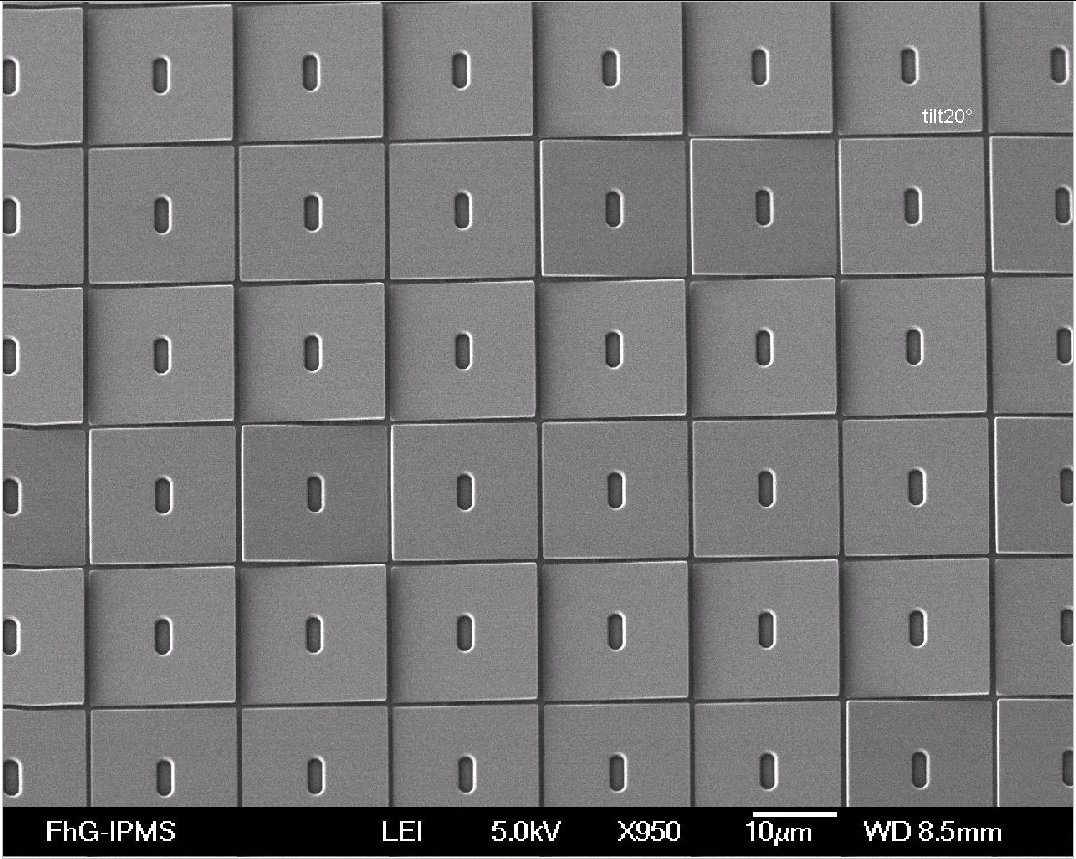
\includegraphics[width=7cm]{mma-tilts}
  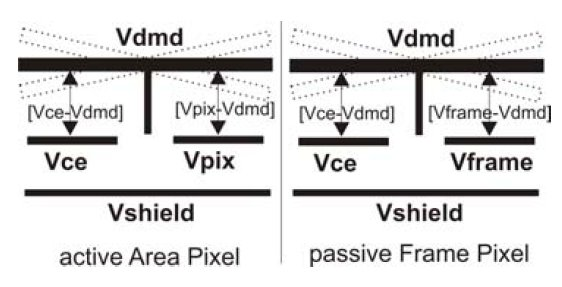
\includegraphics[width=7cm]{mma-voltages}
  \caption{{\bf left:} Electron micrograph showing generation-2 MMA
    with tilted mirrors. {\bf right:} Schematic of the voltages on one
    mirror (both figures by Fraunhofer IPMS).}
  \label{fig:mma-tilts}
\end{figure}
From the beginning of the project a Fourier filtering--based approach
was planned in order to turn the minute tilts of the micro mirrors
into intensity modulations: An aperture is placed on the zero order of
the Fraunhofer diffraction pattern of the MMA. When mirrors are
tilted, they reflect the light outside of the aperture, where it is
absorbed.

However, the Fourier filtering approach has a drawback: The
illumination angles and the size of the aperture are restricted below
the diffraction angles of the MMA. In our optical system this limits
the area on the LCoS, that can be illuminated and therefore the field
of view in the specimen.

A shearing interferometer--based approach was suggested
instead. There, the images of neighbouring mirrors are overlapped and
can interfere. A system based on Wollaston (or Nomarski or DIC
(differential interference contrast)) prisms would give better angular
acceptance. It promises good contrast and will work for multiple
wavelengths as well. Here we describe experiments that were conducted
on the generation-0 MMA with a set of Nomarski prisms from a Zeiss
differential interference contrast microscope.
\section{Description of the setup}
\begin{figure}[ht]
  \centering
  %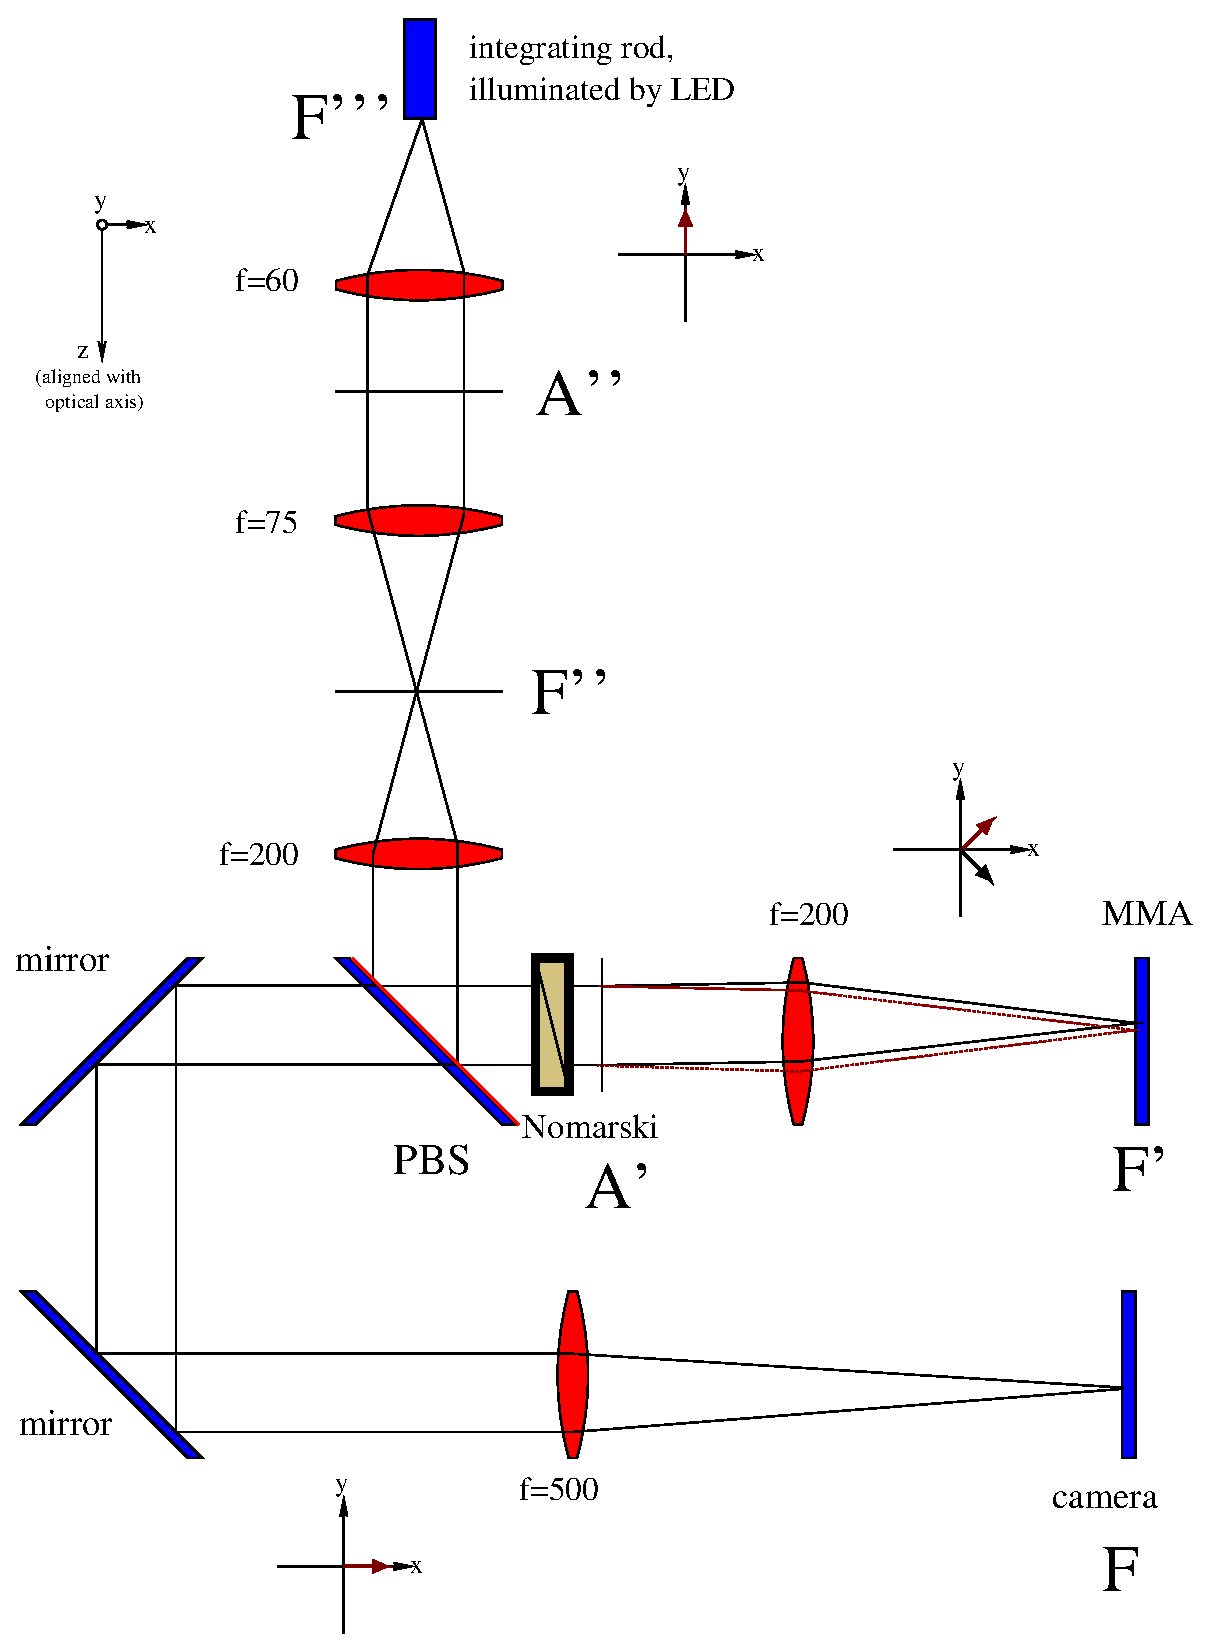
\includegraphics[height=9cm]{../app_dic/img/dic_mma}
  \input{dic_mma.eps_tex} % w=87.6mm
  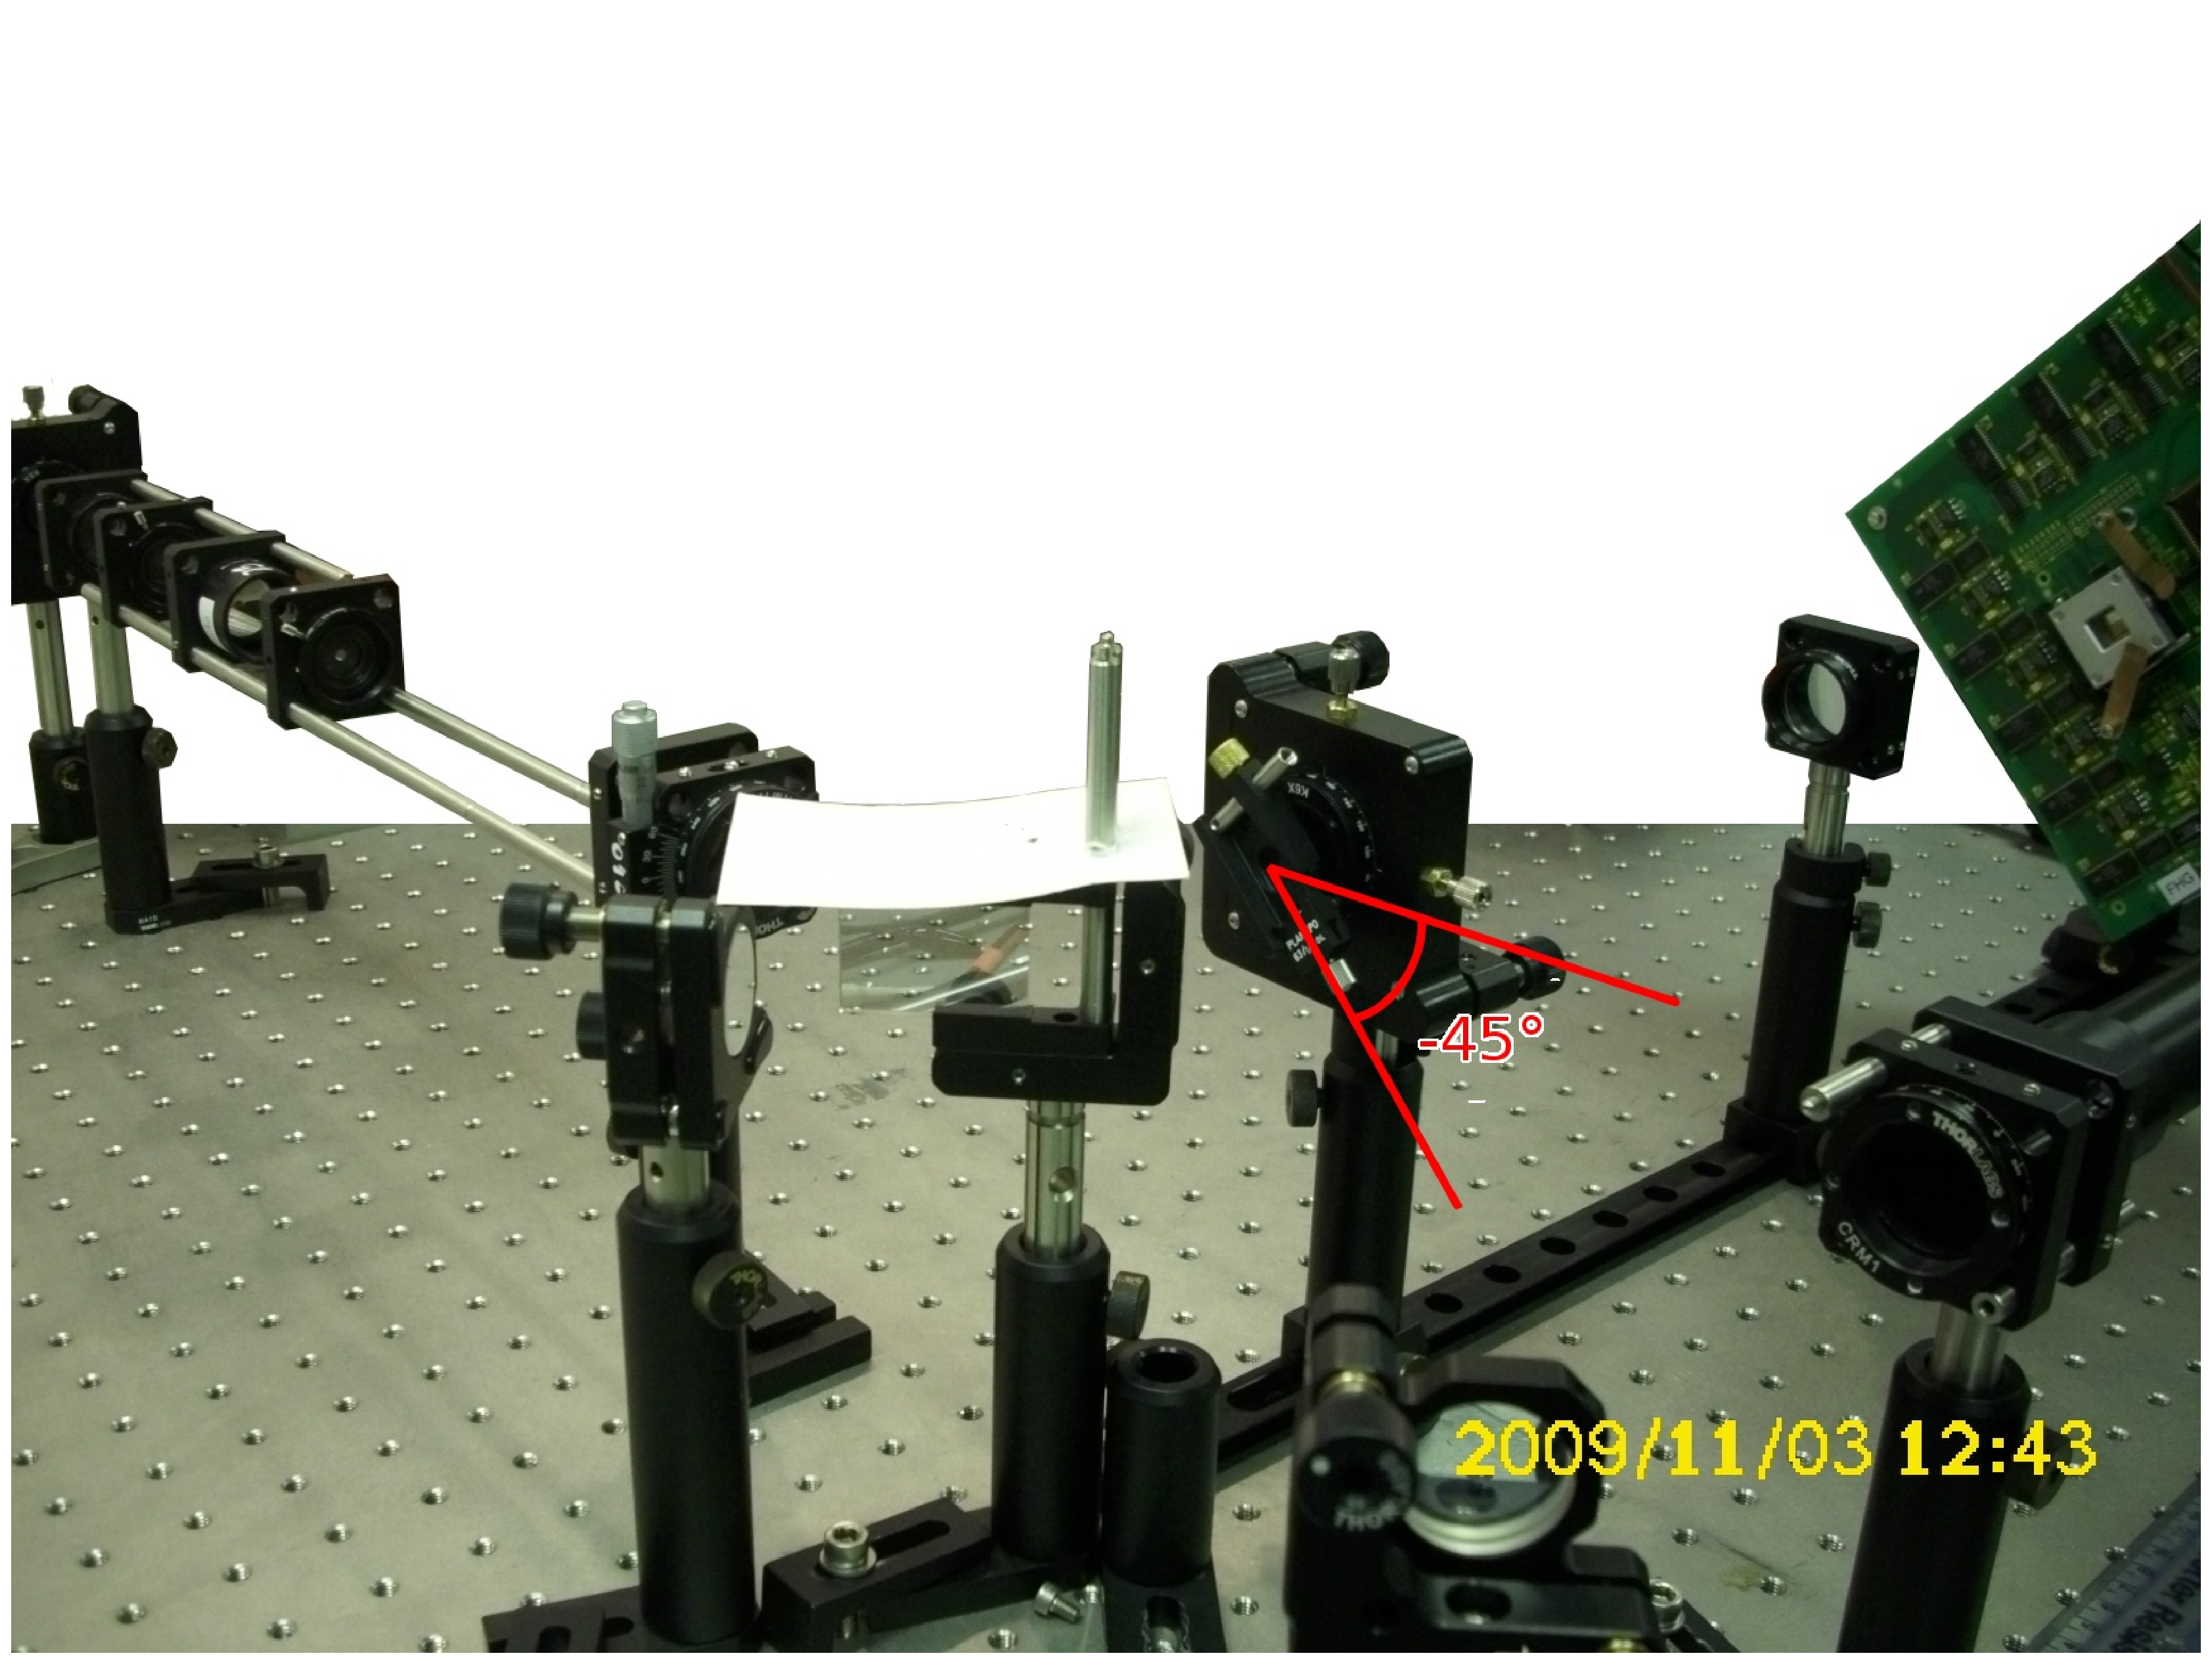
\includegraphics[width=6cm]{../app_dic/img/dsci1331}
  \caption{ Schematic and photograph of the optical setup.  {\bf
      left:} Apertures allow control of the illumination in the planes
    $A''$ and $F''$. The wire grid polarizing beam splitter (PBS) is
    oriented with the aluminium structured side towards the Nomarski
    prism. The Nomarski prism can be rotated around the optical
    axis. {\bf right:} Interference of neighbouring micro mirrors is
    expected for the four angular settings ($\pm 45^\circ$, $\pm
    135^\circ$) of the Nomarski prism.  Here the Nomarski prism is
    oriented in $-45^\circ$ direction.  A white paper card protects
    the wire grid polarizer from dust.  This setup contains two
    additional cleanup polarizers that are not shown in the
    schematic.}
  \label{fig:dic_mma}
\end{figure}
\figref{fig:dic_mma} shows a schematic and a photograph of the setup.
The light source is a liquid light guide--coupled \unit[480]{nm} LED
(CoolLed). It illuminates a square integration rod (\unit[10]{cm}
length) to provide a uniform light distribution in the conjugate
$F'''$ of the field. \nomenclature{DIC}{differential interference contrast}

The optical path for the illumination contains two apertures to
confine the field and to control the illumination angles. We use a
wire grid polarizer (Moxtek, UT, US) as polarizing beam splitter.
Achromatic doublets (objective $f=\unit[200]{mm}$, tube lens
$f=\unit[500]{mm}$) were used as the two imaging lenses.

The position of the focal plane of the Nomarski prisms was estimated
by measuring the distance between the prism and the back focal plane
of the matching micro objectives (the result is generally within
$\unit[2-3]{cm}$). For a flat sample (all MMA mirrors undeflected) we
see a dark band in the interference image. Moving the prism along the
optical axis expands the dark band until it encompasses the full field
of view. We used this to adjust the precise position of the prism.

We selected the prism with the biggest split angle
($\theta=\unit[0.078]{mrad}$, the matching prism for a $63\times/1.4$
oil immersion objective, see section \ref{sec:prism} for the
measurement) in order to keep the distances small and minimize beam
distortion due to air fluctuations. Later we found that the free
aperture of the prism is the limiting factor. For a good DIC effect at
least three orders of the MMA diffraction pattern have to pass through
the prism. Otherwise the prism acts as a Fourier filter. Then the
combined effect of Fourier filtering and (only partial) differential
interference greatly diminishes the contrast of the image.

To reduce the Fourier filtering effect, two identical Nomarski prisms
with \unit[0.078]{mrad} split angle were placed into the setup instead
of one (see \figref{fig:double-prism}). Then we used an objective lens
with shorter focal length. Later we learned that the distance between
the prisms allows to vary the split angle \citep{Schwertner2008}.


\begin{figure}[htb]
  \centering
  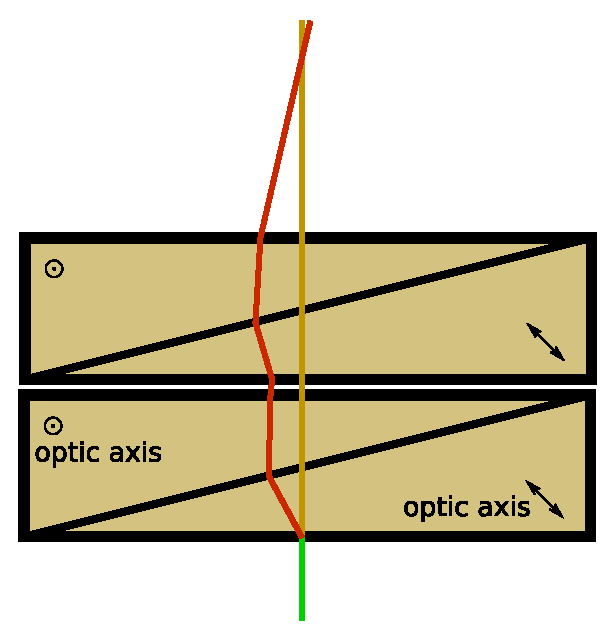
\includegraphics[width=5cm]{../app_dic/img/double-prism}
  \caption{Combination of two identical Nomarski prisms to increase
    the split angle between ordinary and extraordinary beam. The prism
    in the experiments are for a $63\times/1.4$ oil immersion
    objective.}
  \label{fig:double-prism}
\end{figure}

\section{Experiments}
\subsection{Procedure to measure the split angle of a Nomarski prism}
\label{sec:prism}
An important task in the beginning was to measure the split angle of
the various Nomarski prisms in our set. The goal was to find a prism
that with a standard lens would give a shear distance equal to the
mirror pitch of the MMA (\unit[16]{$\mu$m}).

The Nomarski prism consists of two quartz wedges. Its function is
based on the birefringence of the crystal. The prism splits a
$45^\circ$ linearly polarized wavefront into two wavefronts with
slightly diverging angles.
\begin{figure}[htb]
  \centering
  \includegraphics[width=8cm]{../app_dic/img/nomarski_split}
  \caption{Setup to measure the split angle $\theta$ of a Nomarski
    prism by interference of the two beams. The polarizers Pol1 and
    Pol2 are crossed and in a $45^\circ$ angle relative to the shift
    axis of the prism.}
  \label{fig:nomarski_split}
\end{figure}
The split is so small that its direct measurement --- illuminating the
prism with a parallel beam and putting the camera into the back focal
plane of a lens with a long focal length --- is difficult.  Instead we
put the prism between crossed polarizers, illuminate it with a
parallel beam and measure a fringe pattern on the camera (see
\figref{fig:nomarski_split} for a schematic of the setup and
\figref{fig:nomarski_split_exp} for the data).

The electrical field $U$ after the second polarizer is:
\begin{align}
  U&=e^{i\vect k_1\vect r}+e^{i\vect k_2\vect r},\\
  \abs{\vect k}&=\frac{2\pi}{\lambda},\\
  \vect k_1&=\abs{\vect k}(0, \hspace{1em}\sin(\theta/2), \cos(\theta/2))^T,\\
  \vect k_2&=\abs{\vect k}(0, -\sin(\theta/2), \cos(\theta/2))^T.
\end{align}
The camera measures the intensity $I$:
\begin{align}
  I=\abs{U}^2=4\cos^2(\abs{\vect k}y\sin(\theta/2)).
\end{align}
Therefore the dark bands have a distance $d$ (for small split angles
$\theta$):
\begin{align}
  d=\frac{\lambda}{2\sin{\theta/2}}\approx \frac{\lambda}{\theta}.
\end{align}
\begin{figure}[htb]
  \centering
  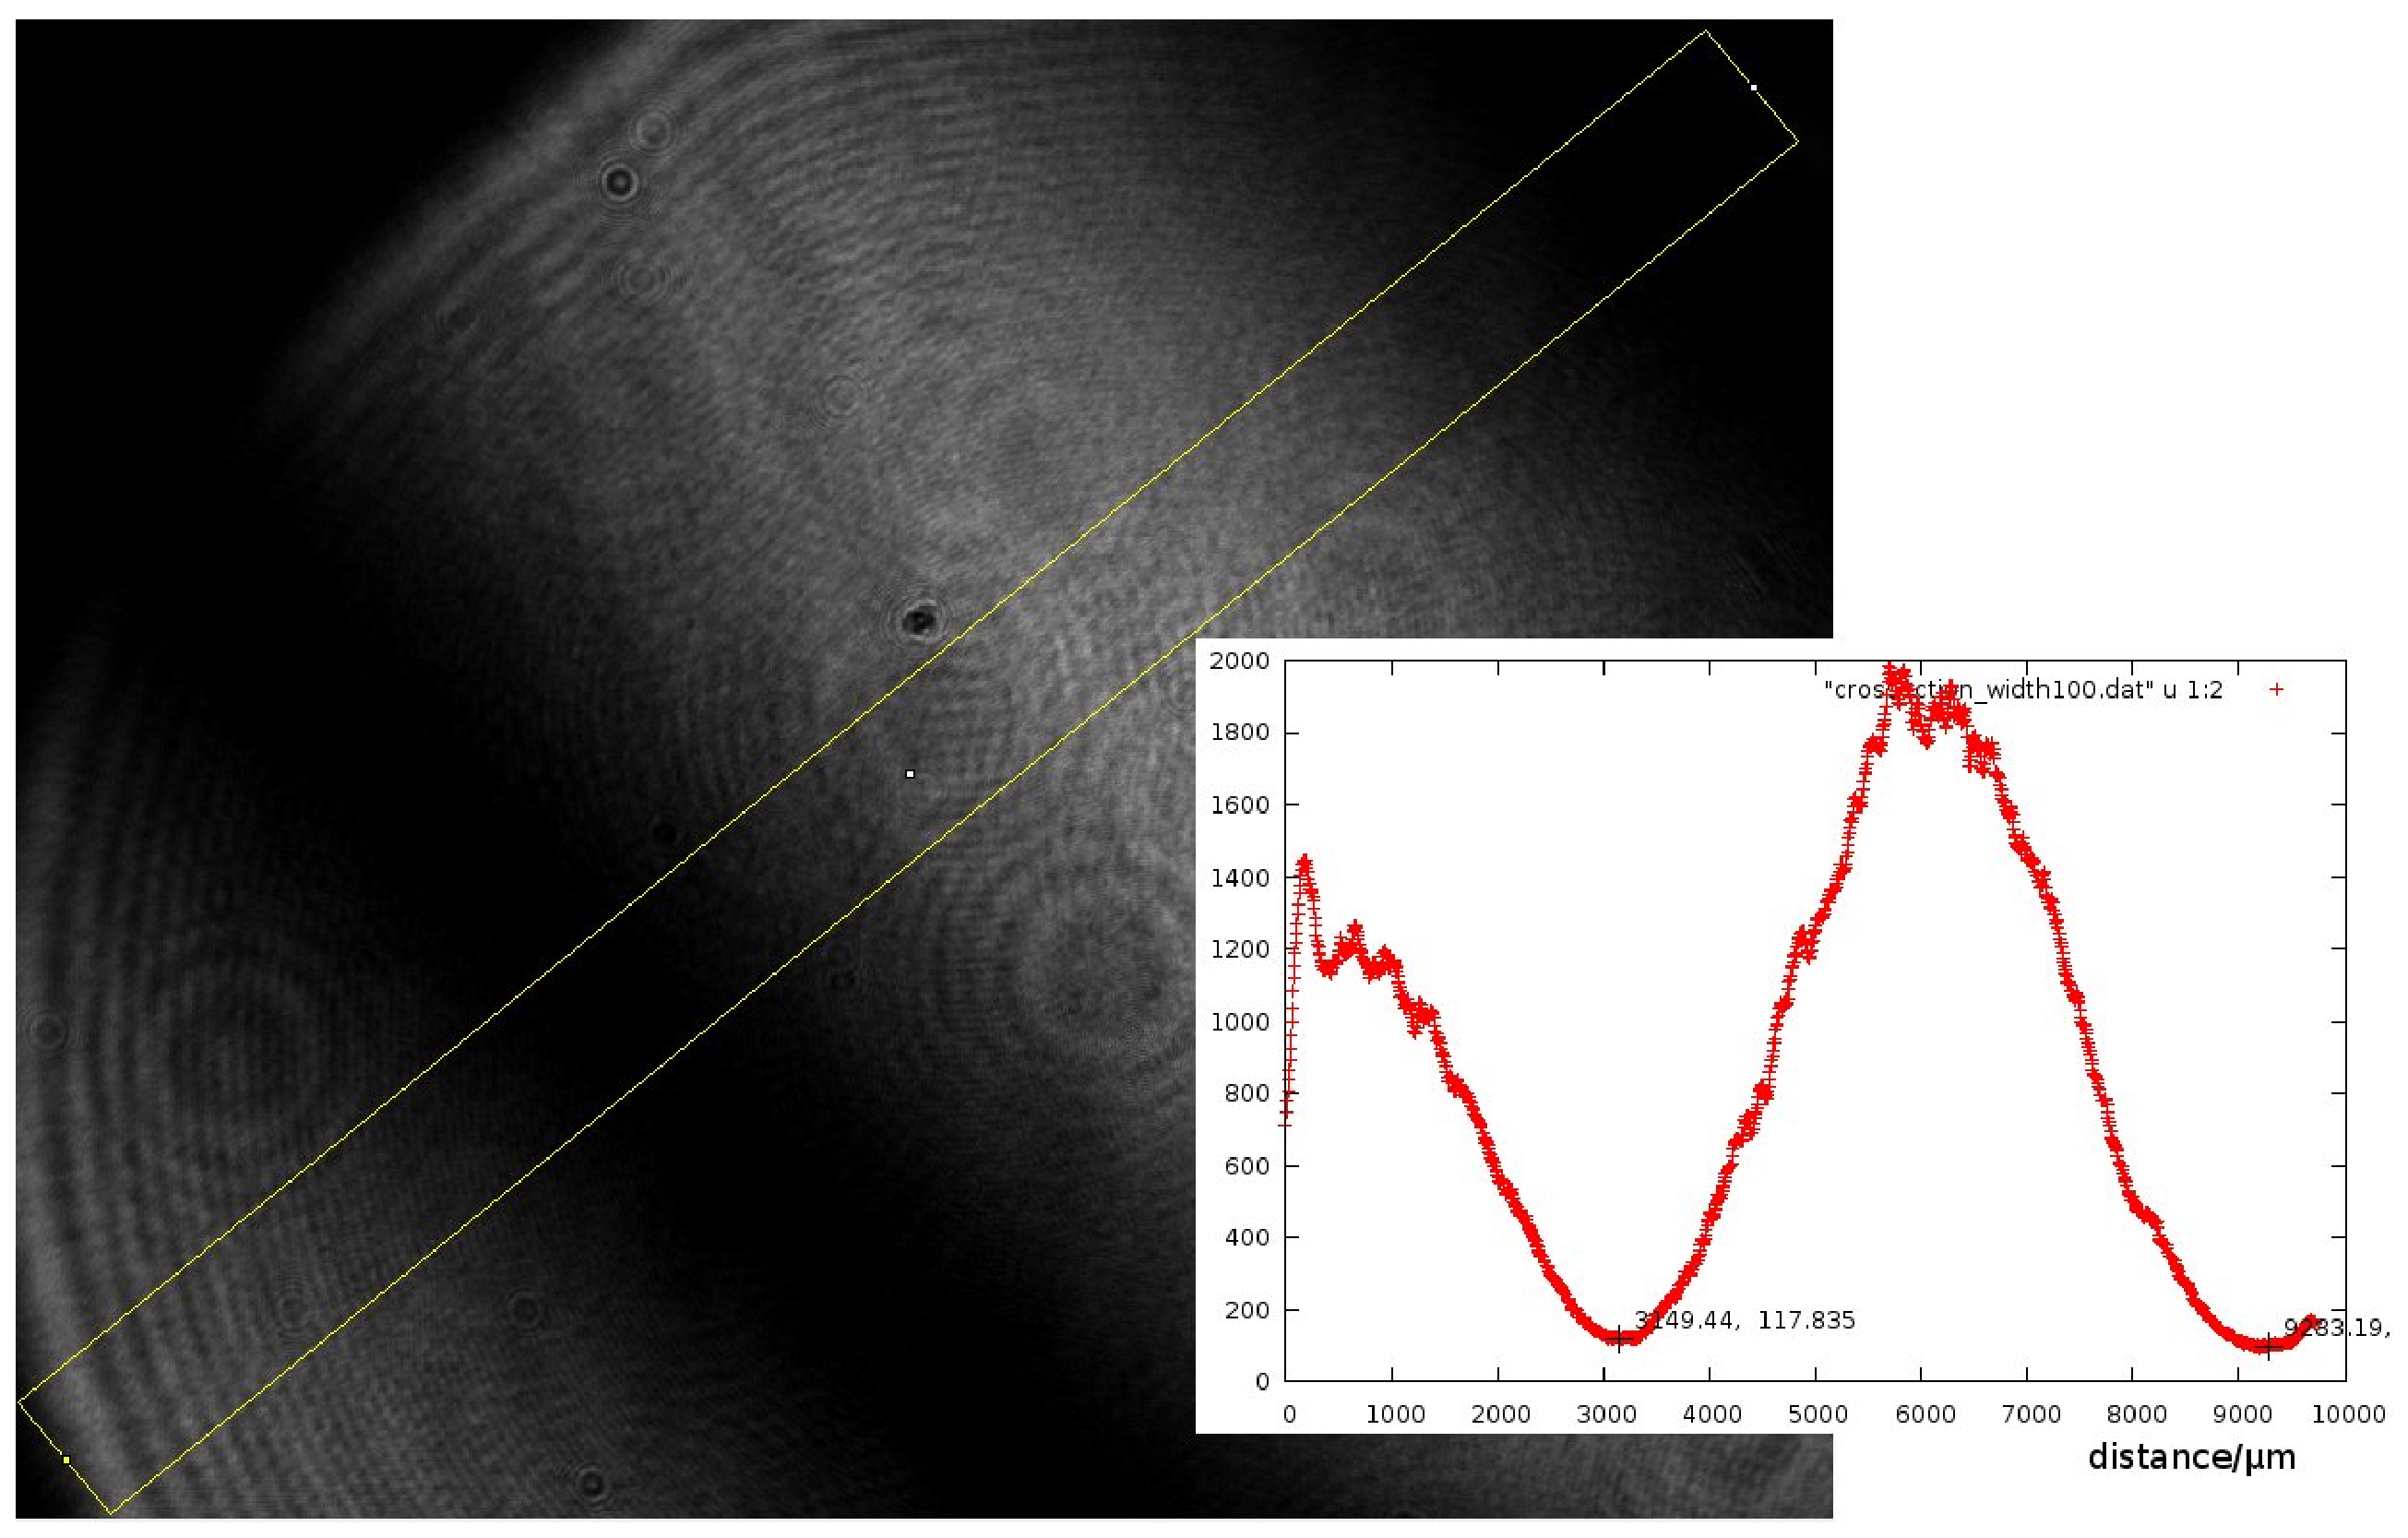
\includegraphics[width=10cm]{../app_dic/img/nomarski_split_exp}
  \caption{Camera image for the prism with the biggest split
    angle. The distance between the two dark fringes is
    $d=\unit[(6.06\pm0.08)]{mm}$. The light source is a laser with
    \unit[473]{nm} wavelength. For the graph, values were integrated
    over the width of the yellow bar to reduce the influence of the
    disturbing fringes.}
  \label{fig:nomarski_split_exp}
\end{figure}
We measured $d=\unit[(6.06\pm0.08)]{mm}$ for the strongest of our
Nomarski prisms.  Other prisms had very small split angles and no two
dark bands could be observed over their clear aperture.

The measured prism has a split angle of $\theta=\unit[0.078]{mrad}$.  For
a lens with a focal distance $f=\unit[200]{mm}$ this corresponds to a
Nomarski split $\Delta x$:
\begin{align}
  \Delta x=2f\tan(\theta/2)\approx f\theta=\unit[(15.6\pm0.2)]{\mu m}.
\end{align}
This is close to the pixel pitch of $\unit[16]{\mu m}$ of the MMA.

\subsection{Imaging the MMA with the DIC method}
\figref{fig:screen5} shows two typical images that can be obtained in
the DIC setup. The schematic in \figref{fig:screen} indicates the
shearing direction and corresponding interference pattern.  For both
images a checkerboard pattern with a periodicity of $16\times16$
elements is displayed on the MMA.

In the right image (\figref{fig:screen} right,
\figref{fig:screen5}~b)) the interference occurs between mirrors that
tilt in different directions (green in the schematic).

Areas on the checkerboard pattern with deflected mirrors appear bright
in the image, regions with flat mirrors are dark. On two edges of the
checkerboard square tilted mirros interfer with flat ones, resulting
in dimmer pixels in the interference image (indicated by purple arrow
in bottom right of \figref{fig:screen5}).

In this configuration it is not possible to produce a perfectly dark
interference next to a deflected mirror.  Therefore, with this shear
direction we cannot display arbitrary gray value images with the
torsion micro mirrors of the MMA.


\begin{figure}[ht]
  \centering
  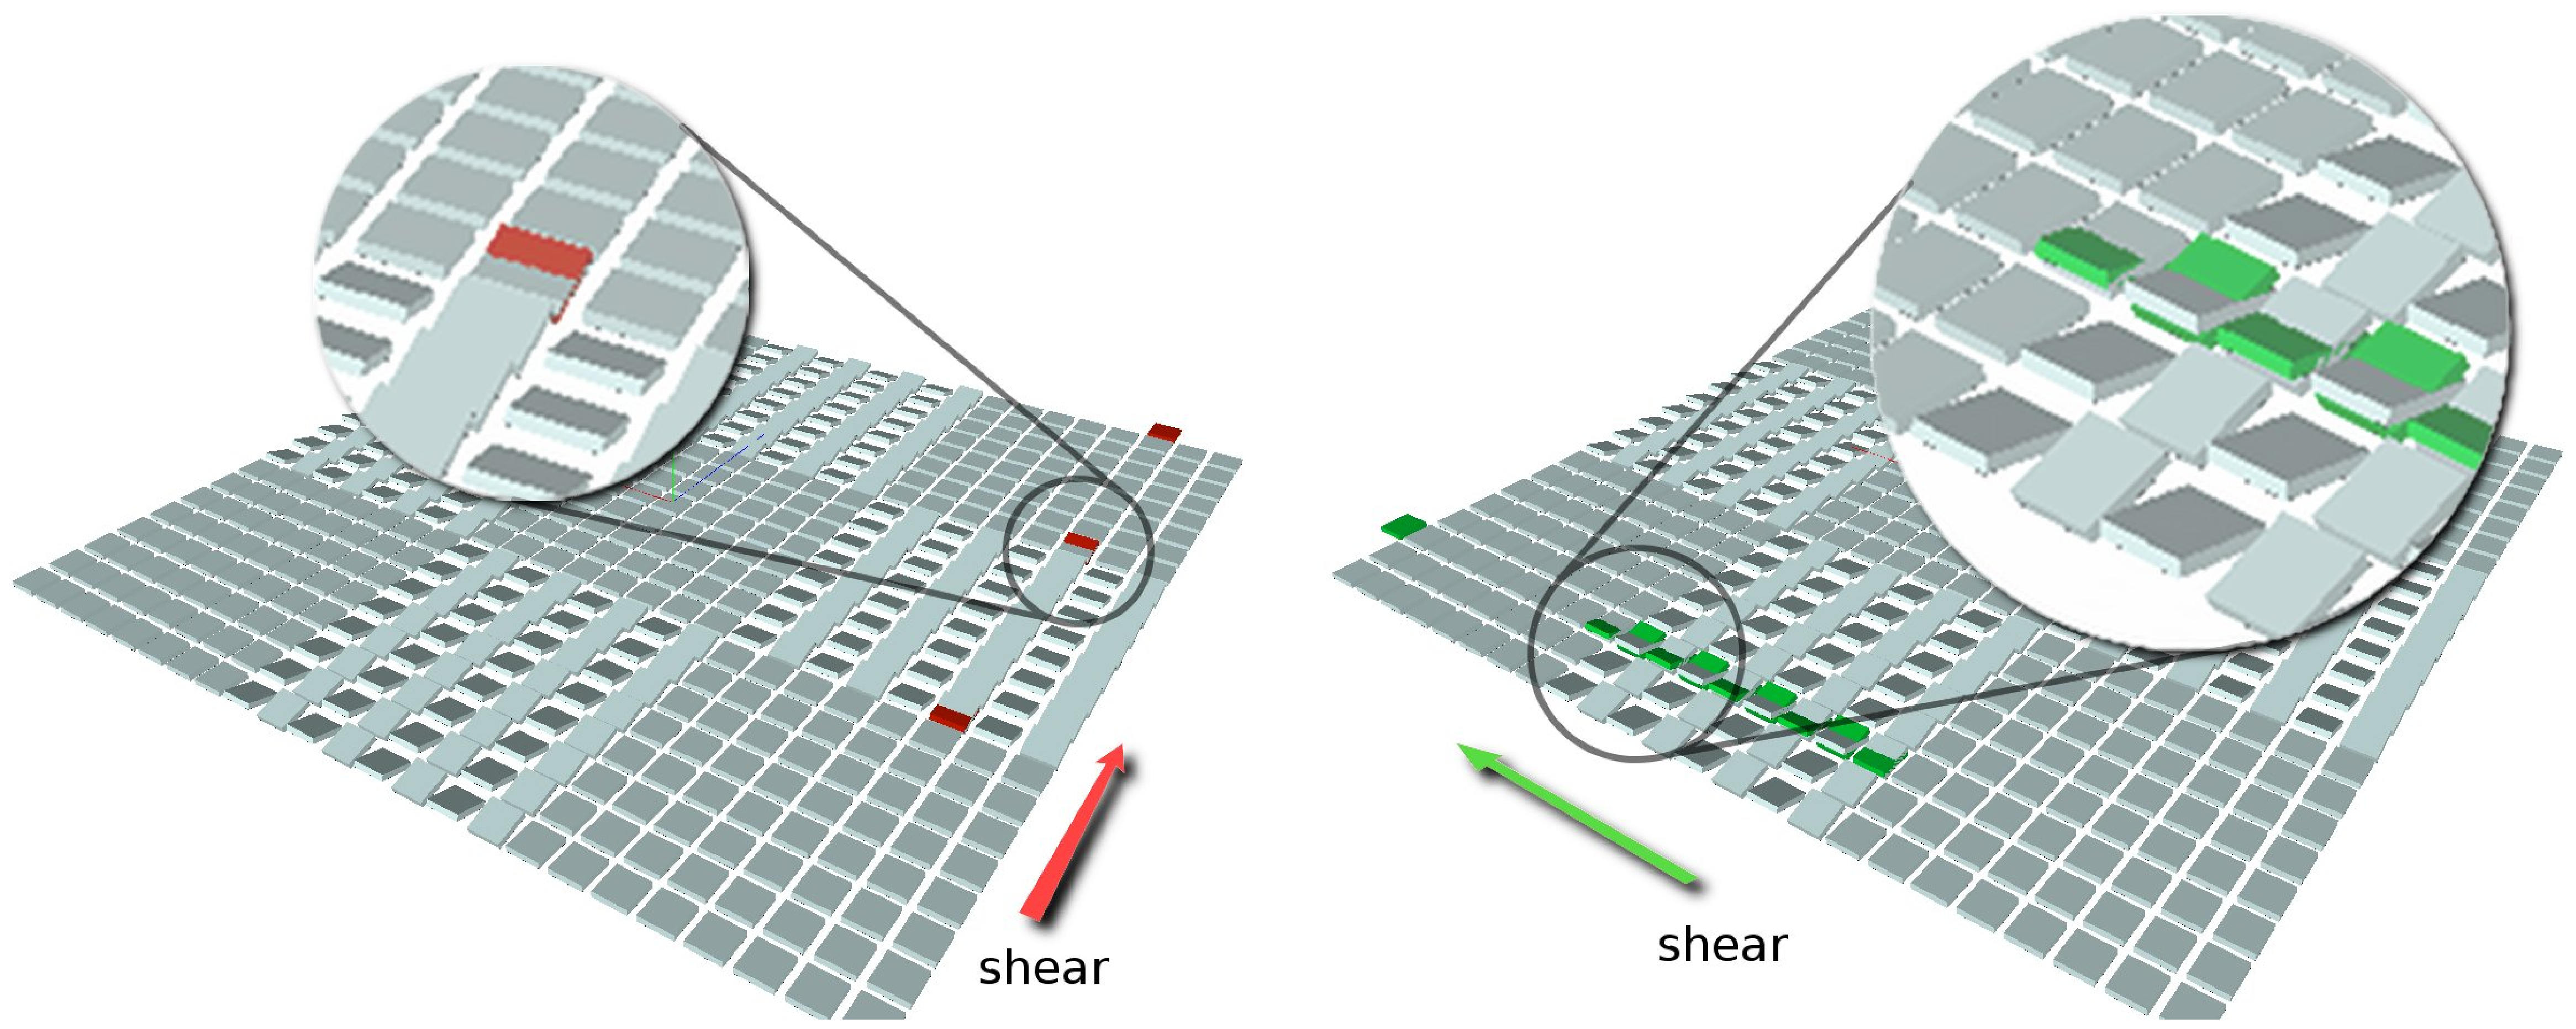
\includegraphics[width=\linewidth]{../app_dic/img/mma_sketch}
  \caption{Schematic showing how neighbouring mirrors are overlaid by
    the Nomarski prism. $24\times 24$ region of micro mirrors that
    display a checkerboard of $16\times 16$ periodicity. Colour
    indicates neighbouring micro mirrors, that will give rise to
    non-destructive interference in the images on the camera. {\bf
      left:} Prism in $-45^\circ$ orientation. {\bf right:} Prism in
    $+45^\circ$ orientation.}
  \label{fig:screen}
\end{figure}

\begin{figure}[!htbp]
  \centering
  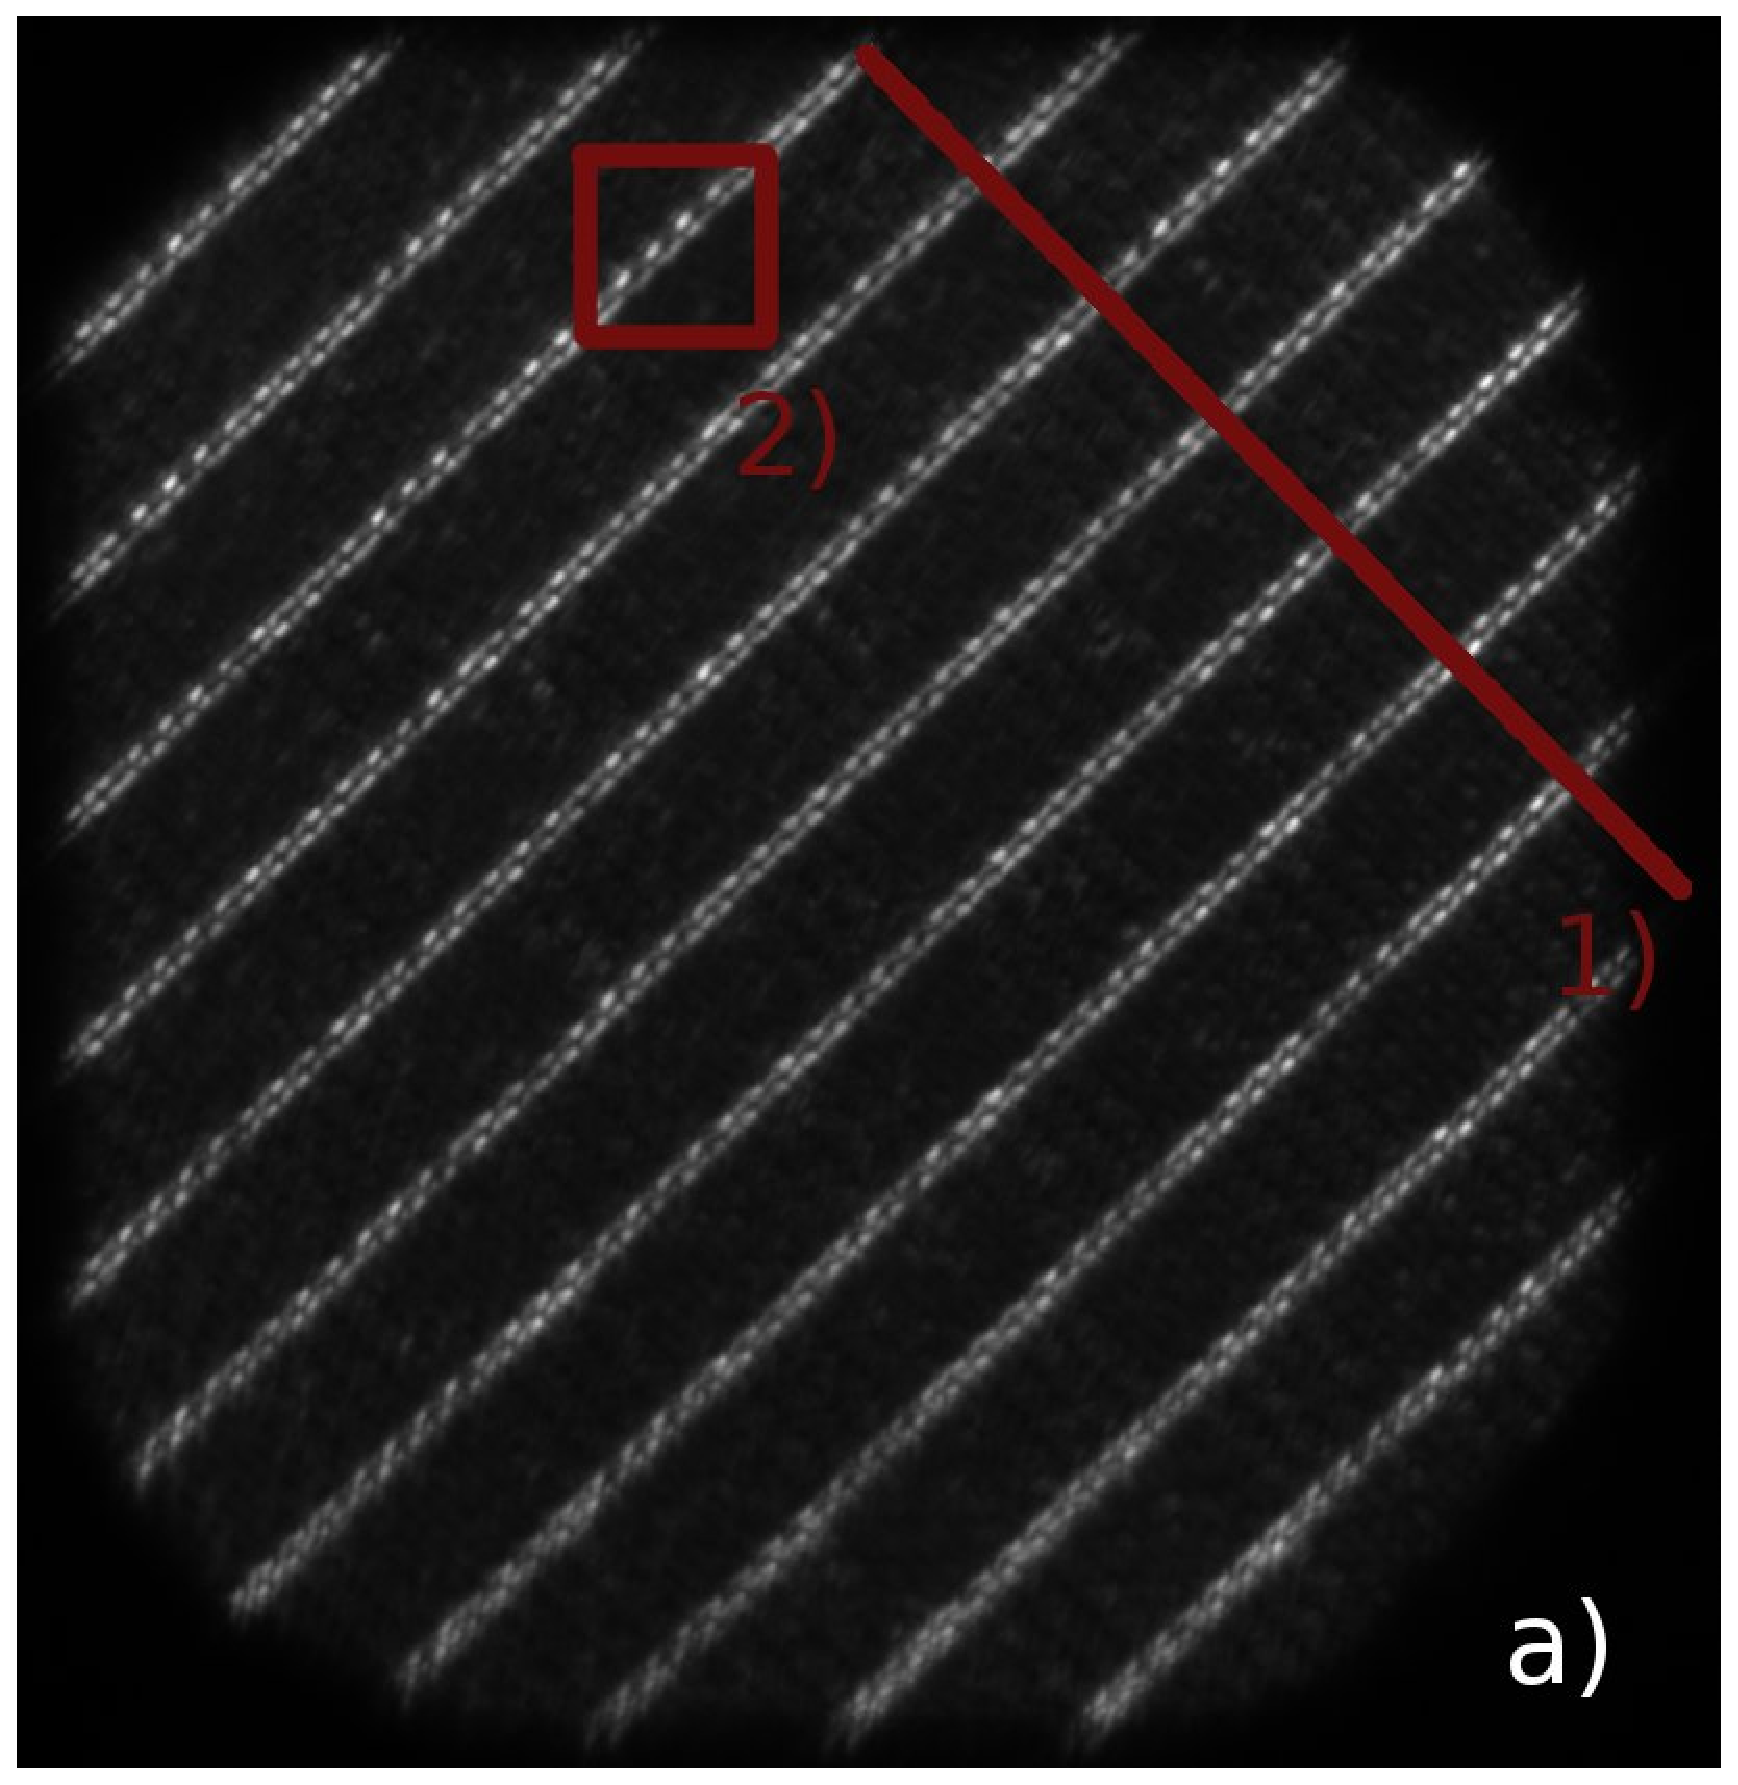
\includegraphics[height=5.9cm]{../app_dic/img/1219/auswert/1checker}
  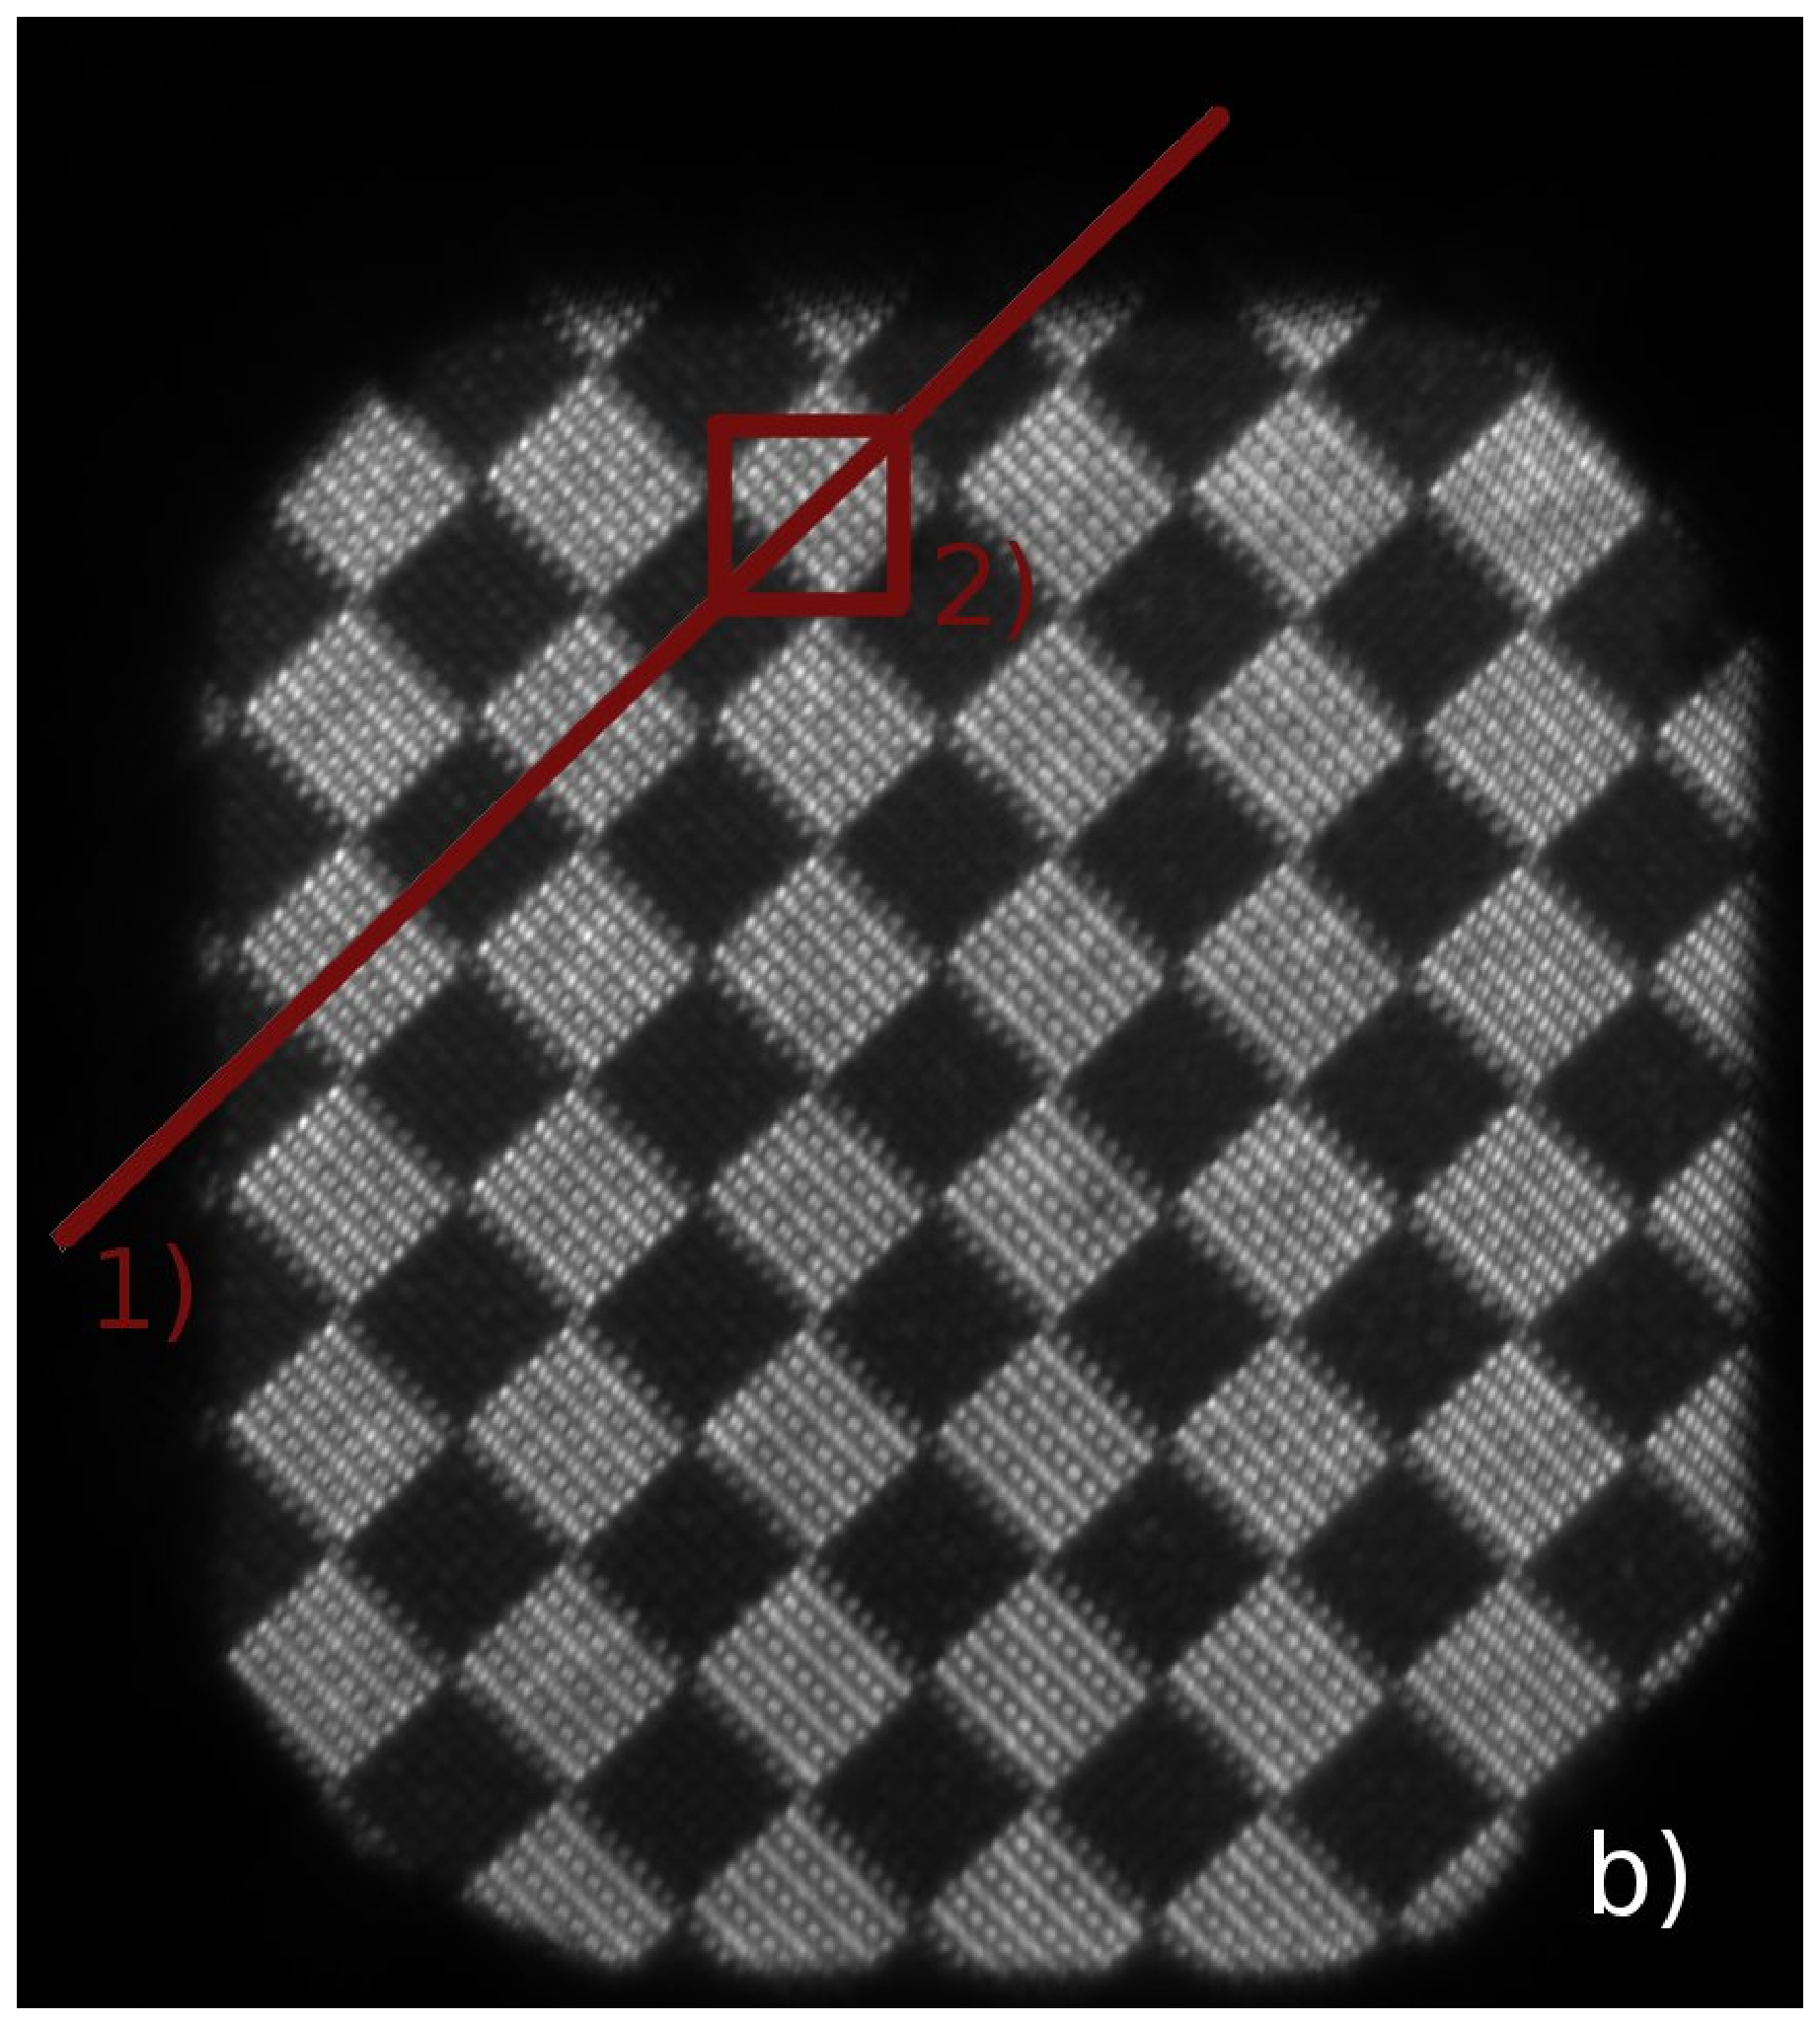
\includegraphics[height=5.9cm]{../app_dic/img/1219/auswert/2checker}
  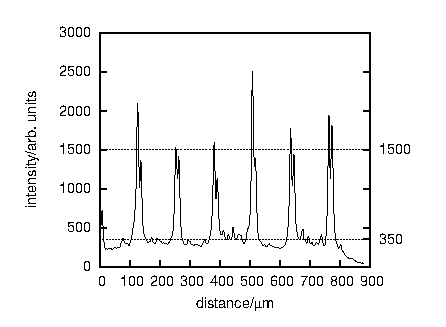
\includegraphics[width=7cm]{../app_dic/img/1219/auswert/1checker-section}
  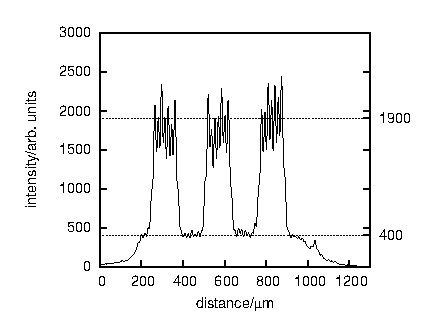
\includegraphics[width=7cm]{../app_dic/img/1219/auswert/2checker-section}
  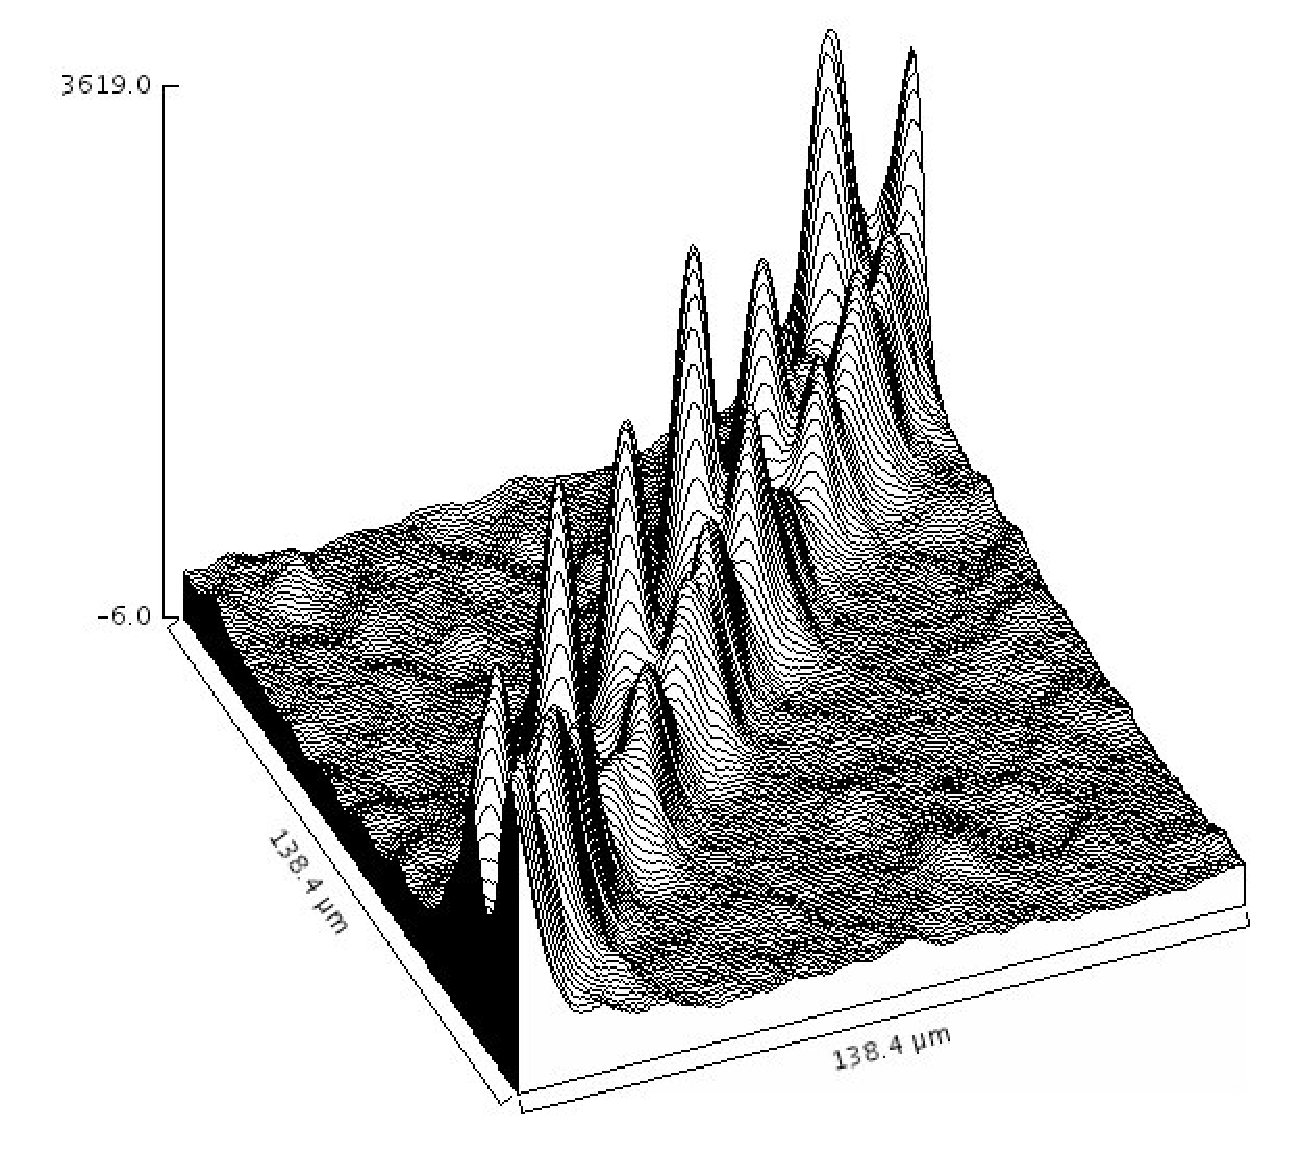
\includegraphics[width=7cm]{../app_dic/img/1219/auswert/1checker-height}
  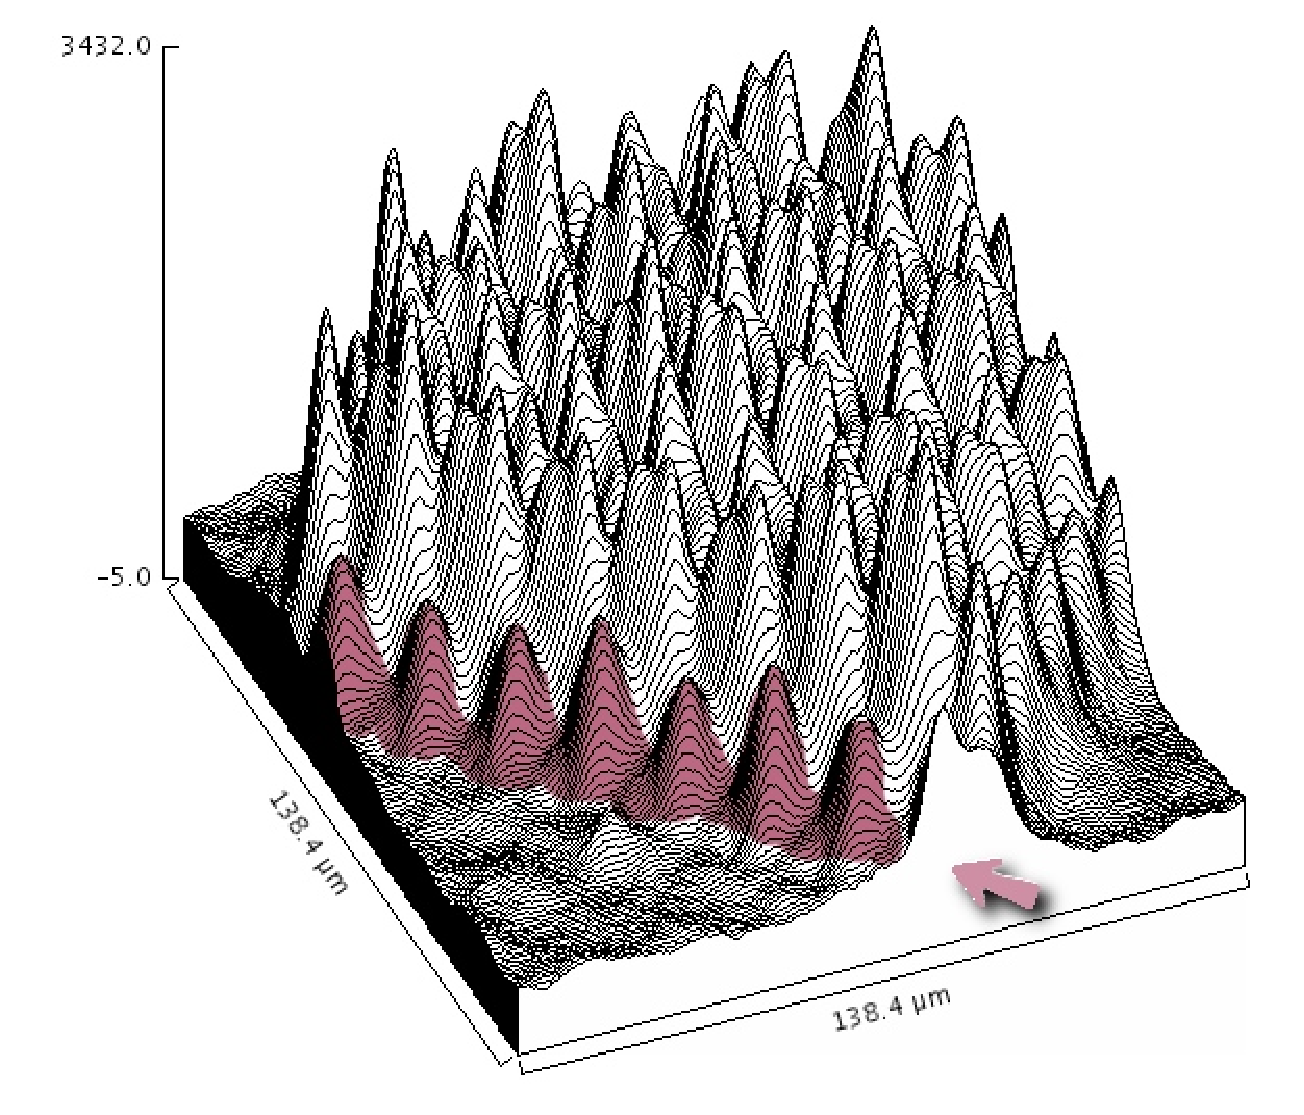
\includegraphics[width=7cm]{../app_dic/img/1219/auswert/2checker-height-arrow}
  \caption{{\bf top:} DIC image for a prism setting of $-45^\circ$ (a)
    and $+45^\circ$ (b) (see \figref{fig:screen} for a
    schematic). {\bf middle:} Cross section along the DIC shift
    direction (line marked with 1). {\bf bottom:} Zoom into boxes
    (marked with 2) in the images.  Both DIC images were obtained 
    with two identical sequential DIC prisms (for $63\times/1.4$), a
    \unit[100]{mm} objective lens and a \unit[300]{mm} tube lens.}
  \label{fig:screen5}
\end{figure}

In the other shear direction (\figref{fig:screen} left,
\figref{fig:screen5}~a)) mirrors, that tilt into the same direction,
are brought to interference. Neighbouring mirrors that have the same
deflection result in a black interference image. 

For a bright value in the interference image, both mirrors must be
deflected to a different angle. The closer the two neighbours are in
their deflection angle, the darker their interference image will be.
Therefore it is possible to display arbitrary gray value images in
this configuration.

\subsubsection*{Displaying arbitrary gray value images}

For this, we devised an algorithm that assigns a deflection $d_0$ to
the mirrors on one side of the display and then iterates through the
rows of the goal image that is going to be displayed. For each mirror
$i$ along the row its deflection $d_i(d_{i-1},E_i)$ is calculated in
dependence of the deflection $d_{i-1}$ of the previous mirror and the
goal energy $E_i$ in this pixel.

In the next section we develop a forward model to calculate the energy
$E_i(d_i-d_{i-1})$ of one pixel depending on the deflection difference
between neighbouring mirrors. Using this model we calculate a look-up
table that we invert and use in the algorithm to find the deflections
$d_i$.


\subsection{Forward model for the energy in the interference image}
\begin{figure}[htb]
  \centering
  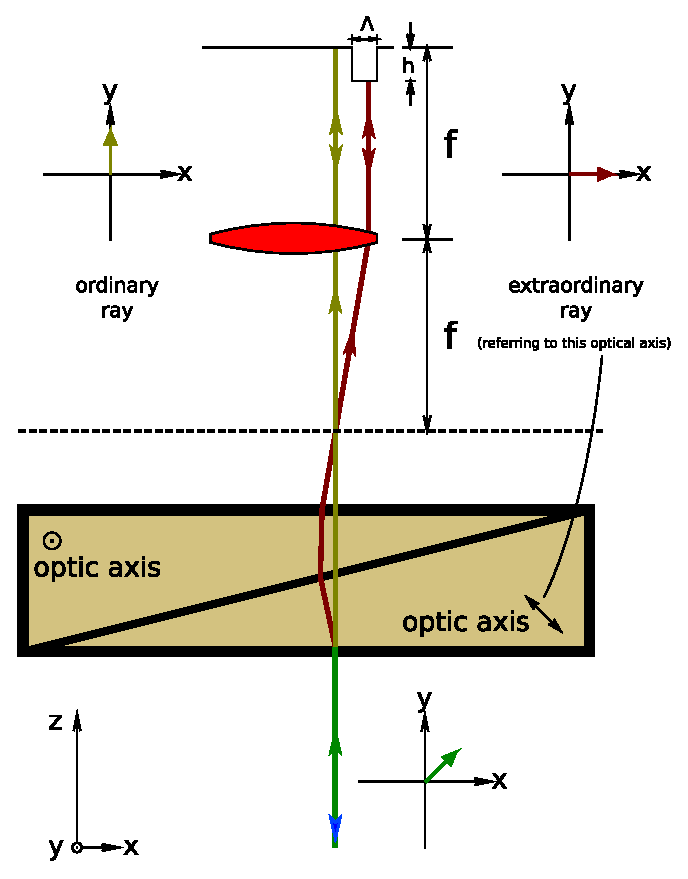
\includegraphics[width=6cm]{../app_dic/img/dic_prism}
  \caption{ Linearly polarized light is split by the prism into two
    rays with slightly diverging angle. They hit the MMA at two spots,
    which are one shearing distance apart. The light returning through
    the Nomarski prism has different polarization states depending on
    the height difference $h$ of the mirrors at those two beam
    positions.}
  \label{fig:prism}
%http://www.microscopy.fsu.edu/primer/java/polarizedlight/crystalwavefronts/index.html
\end{figure}
First we consider the simplified arrangement of one piston micro
mirror of width $\Lambda$ on a plane mirror (see
\figref{fig:prism}). Later we will use the results of this model and
apply them to the torsion mirrors of the MMA (equation
\ref{eqn:it}). 

Let $k=2\pi/\lambda_0$ with vacuum wavelength $\lambda_0$. We write
the influence of a retarder (the height difference $h$ of the small
piston mirror) on a polarized wave in Jones calculus as
(\cite{Goodman1996} p.~418):
\begin{align}
L_r(\Delta)=\begin{pmatrix}1&0\\ 0&e^{-i\Delta}\end{pmatrix}
\end{align}
with a phase difference $\Delta=2kh$ (the factor 2 due to the
reflection).  The matrix for a polarizer that transmits the component
of the electrical field which is linearly polarized at an angle
$\alpha$ to the x-axis is:
\begin{align}
L_p(\alpha)=\begin{pmatrix}\cos^2\alpha&\sin\alpha\cos\alpha\cr
  \sin\alpha\cos\alpha&\sin^2\alpha\end{pmatrix}.
\end{align}
In our setup (see \figref{fig:prism}) the incoming light has a
$45^\circ$ polarization $\vect U=(1,1)^T/\sqrt{2}$ after the first
reflection on the PBS (not shown in the figure, would be in the
bottom). The light traverses the Nomarski prism which splits it into
two diverging beams of orthogonal polarization. A lens collimates the
beams and then they are reflected by the mirror sample. Here,
depending on the height of the piston mirror, a phase retardation is
imposed on one of the two beams. The reflected light is recombined in
the Nomarski prism and only the component that is polarized at
$\alpha=-45^\circ$ passes through the PBS onto the camera: $\vect
U'=L_p(-45^\circ)L_r(\Delta)$.
\begin{align}
  I'=|\vect U'|^2=(1-\cos\Delta)/2
\end{align}
The camera image is dark for a plane mirror and is maximal for a
piston height $h=\lambda/4$.
%a:-%pi/4;
%r:matrix([1,0],[0,exp(-%i*d)]);
%p:matrix([cos(a)^2,sin(a)*cos(a)],[sin(a)*cos(a),sin(a)^2]);
%expand((p . r . [1,1]) . conjugate(p . r . [1,1]));
For a piston mirror of width $\Lambda$ the energy in the corresponding
pixel on the camera is just the intensity times the area:
\begin{align}
  \Delta(x',y') &=2kh=\textrm{const},\\
  E_\textrm{piston}&=\int_{-\Lambda/2}^{\Lambda/2}\int_{-\Lambda/2}^{\Lambda/2}
  I'(\Delta(x',y'))\,\textrm{d}x'\textrm{d}y'=\frac{\Lambda^2}{2}(1-\cos
  \Delta).
\end{align}
\begin{figure}[ht]
  \centering
  \includegraphics[width=7cm]{../app_dic/img/tilt}
  \caption{ Two mirrors with pitch $\Lambda$. Here they are tilted
    with different deflections $d_1$ and $d_2$ in opposite
    directions.}
  \label{fig:tilt}
\end{figure}
As the mirrors of the MMA tilt (and don't move like pistons) it is
necessary solve the integral of the intensity along the DIC shift
direction $x'$ to get the energy in one pixel depending on the tilt of
the two neighbouring mirrors (this calculation is done for small
mirror tilts, see \figref{fig:tilt}):
% Delta = 2kh; 
% integrate((1-cos(2kh))/2,x,-l/2,l/2);
% h(l) = d, h(-l) = d, h(0) = 0
% h(x) = abs(d*x/l) 
% 2*integrate((1-cos(2*k*d*x/l))/2,x,0,l/2);
\begin{align}
\label{eqn:it}
\Delta(x',y') &= 2kh(x') = 2k\frac{\abs{x'} \delta}{\Lambda},\\
E_\textrm{torsion}&=\int_{-\Lambda/2}^{\Lambda/2}\int_{-\Lambda/2}^{\Lambda/2}
I'(\Delta(x',y'))\,
\textrm{d}x'\textrm{d}y'=\frac{\Lambda^2}{2}\left(1-\frac{\sin(k
    \delta)}{k \delta}\right).
\end{align}
Here $\delta=d_1-d_2$ is the difference between the deflections $d_1$
and $d_2$ of the two mirrors and $\Lambda$ is the mirror pitch. If the
deflections $d_1$ and $d_2$ have opposite signs, the mirrors tilt in
opposite directions. Note that the integral sums incoherently across
the mirror because in our experiment we use a LED light source.

Equation \ref{eqn:it} is the forward model. It describes the energy
$E_\textrm{torsion}(d_1-d_2)$ in one pixel of the interference image
depending on the deflections of two neighbouring
mirrors. \figref{fig:erika-detail}~a) shows a gray value image that
should be displayed in the interference image. The corresponding
pattern on the micro mirror array is depicted in b). The image c)
contains the interference image as acquired by the camera.

\begin{figure}[!htbp]
  \centering
  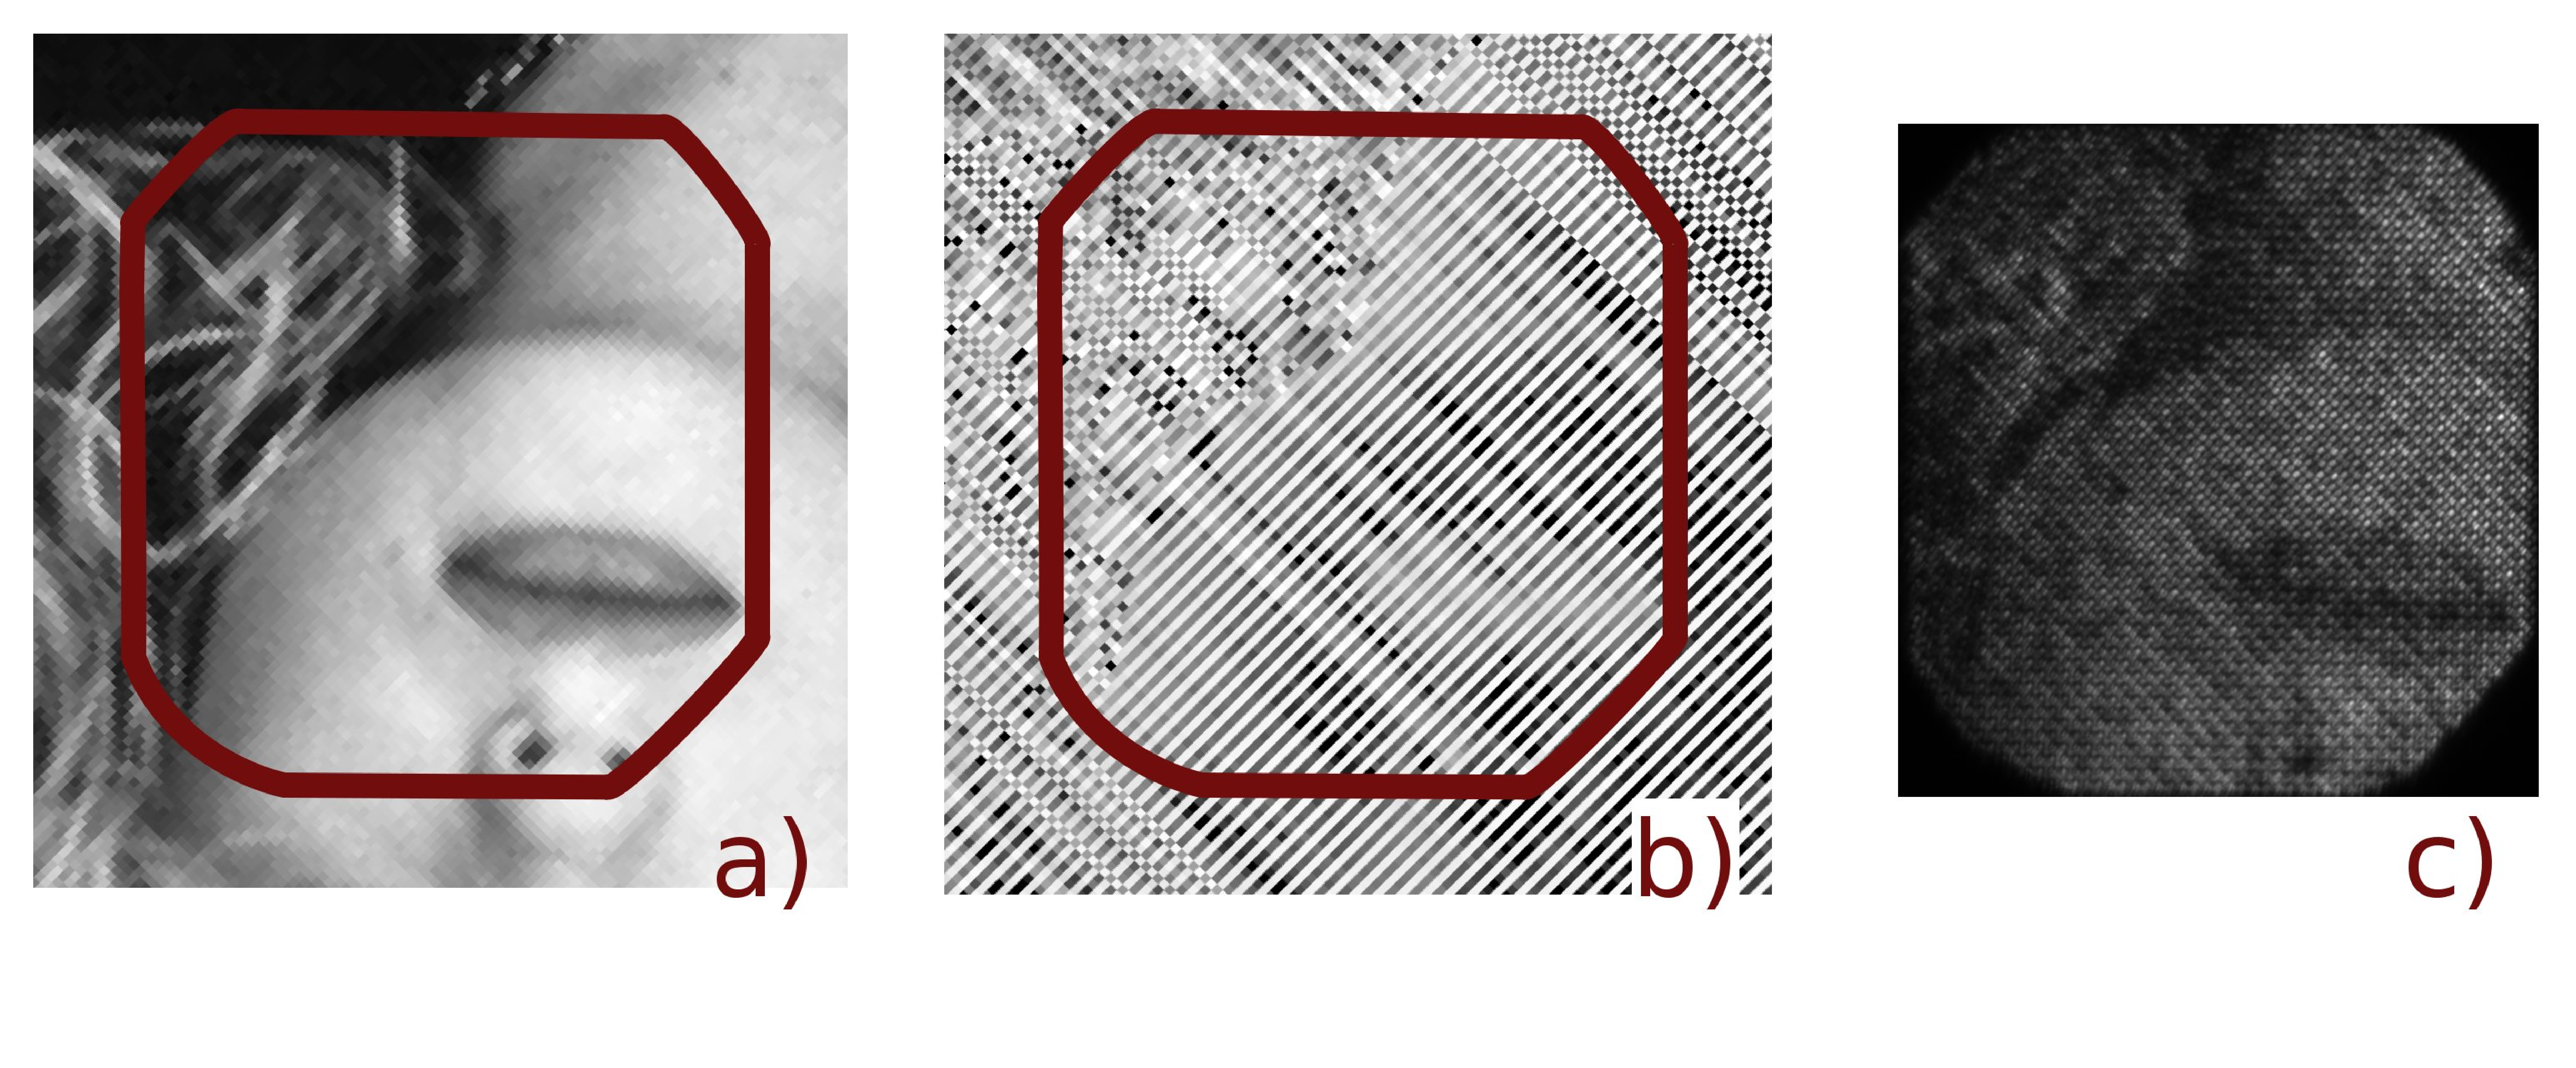
\includegraphics[width=.8\linewidth]{../app_dic/img/1219/auswert/erika-detail}
  \caption{{\bf (a)} Closeup of the input image. {\bf (b)} The
    precomputed (with the look up table algorithm) image that is
    displayed on the MMA. The DIC shift will occur from the left top
    towards the right bottom. Note that regions that are white in the
    input image have a grating structure with high contrast. {\bf (c)}
    The resulting interference image on the camera. For this image we
    used two identical Nomarski prisms in series (for $63\times/1.4$), a
    \unit[100]{mm} objective lens and a \unit[300]{mm} tube lens.}
  \label{fig:erika-detail}
\end{figure}

% sin(a) = m*lambda/Lambda
% asin(473.0/16000) = .0295 rad = 1.694 degree
% tan(a) = r/f -> r = 200 mm * tan(0.0295) = 5.9 mm;
% tan(asin(473/16000))*200

\subsection{Effects of limited prism aperture on DIC image of
  torsional mirrors}
\label{sec:size}
The light coming back from the MMA produces a Fraunhofer diffraction
pattern in the plane $A'$ approximately at the Nomarski prism (see
\figref{fig:dic_mma}). The clear aperture of our prisms is about
\unit[10]{mm}. The first orders due to the \unit[16]{$\mu$m} pixel
pitch of the MMA are at \unit[$\pm5.9$]{mm} with an objective lens of
\unit[200]{mm} focal length.

In order to investigate the influence of the blocking the
$\pm1^\textrm{st}$ orders, we added a circular aperture into plane
$A'$ (\figref{fig:dic_mma}) and captured interference images for
various diameters of this aperture (see \figref{fig:erikas}).  The
schematic above the images depicts the size of the circular aperture
in relation to the diffraction pattern of the MMA.

With decreasing aperture diameter streaks in the images (red arrows)
become more pronounced. These artefacts originate in regions on the
pattern, that is shown on the MMA that differ from their surrounding
rows. 

\begin{figure}[!htb]
  \centering
  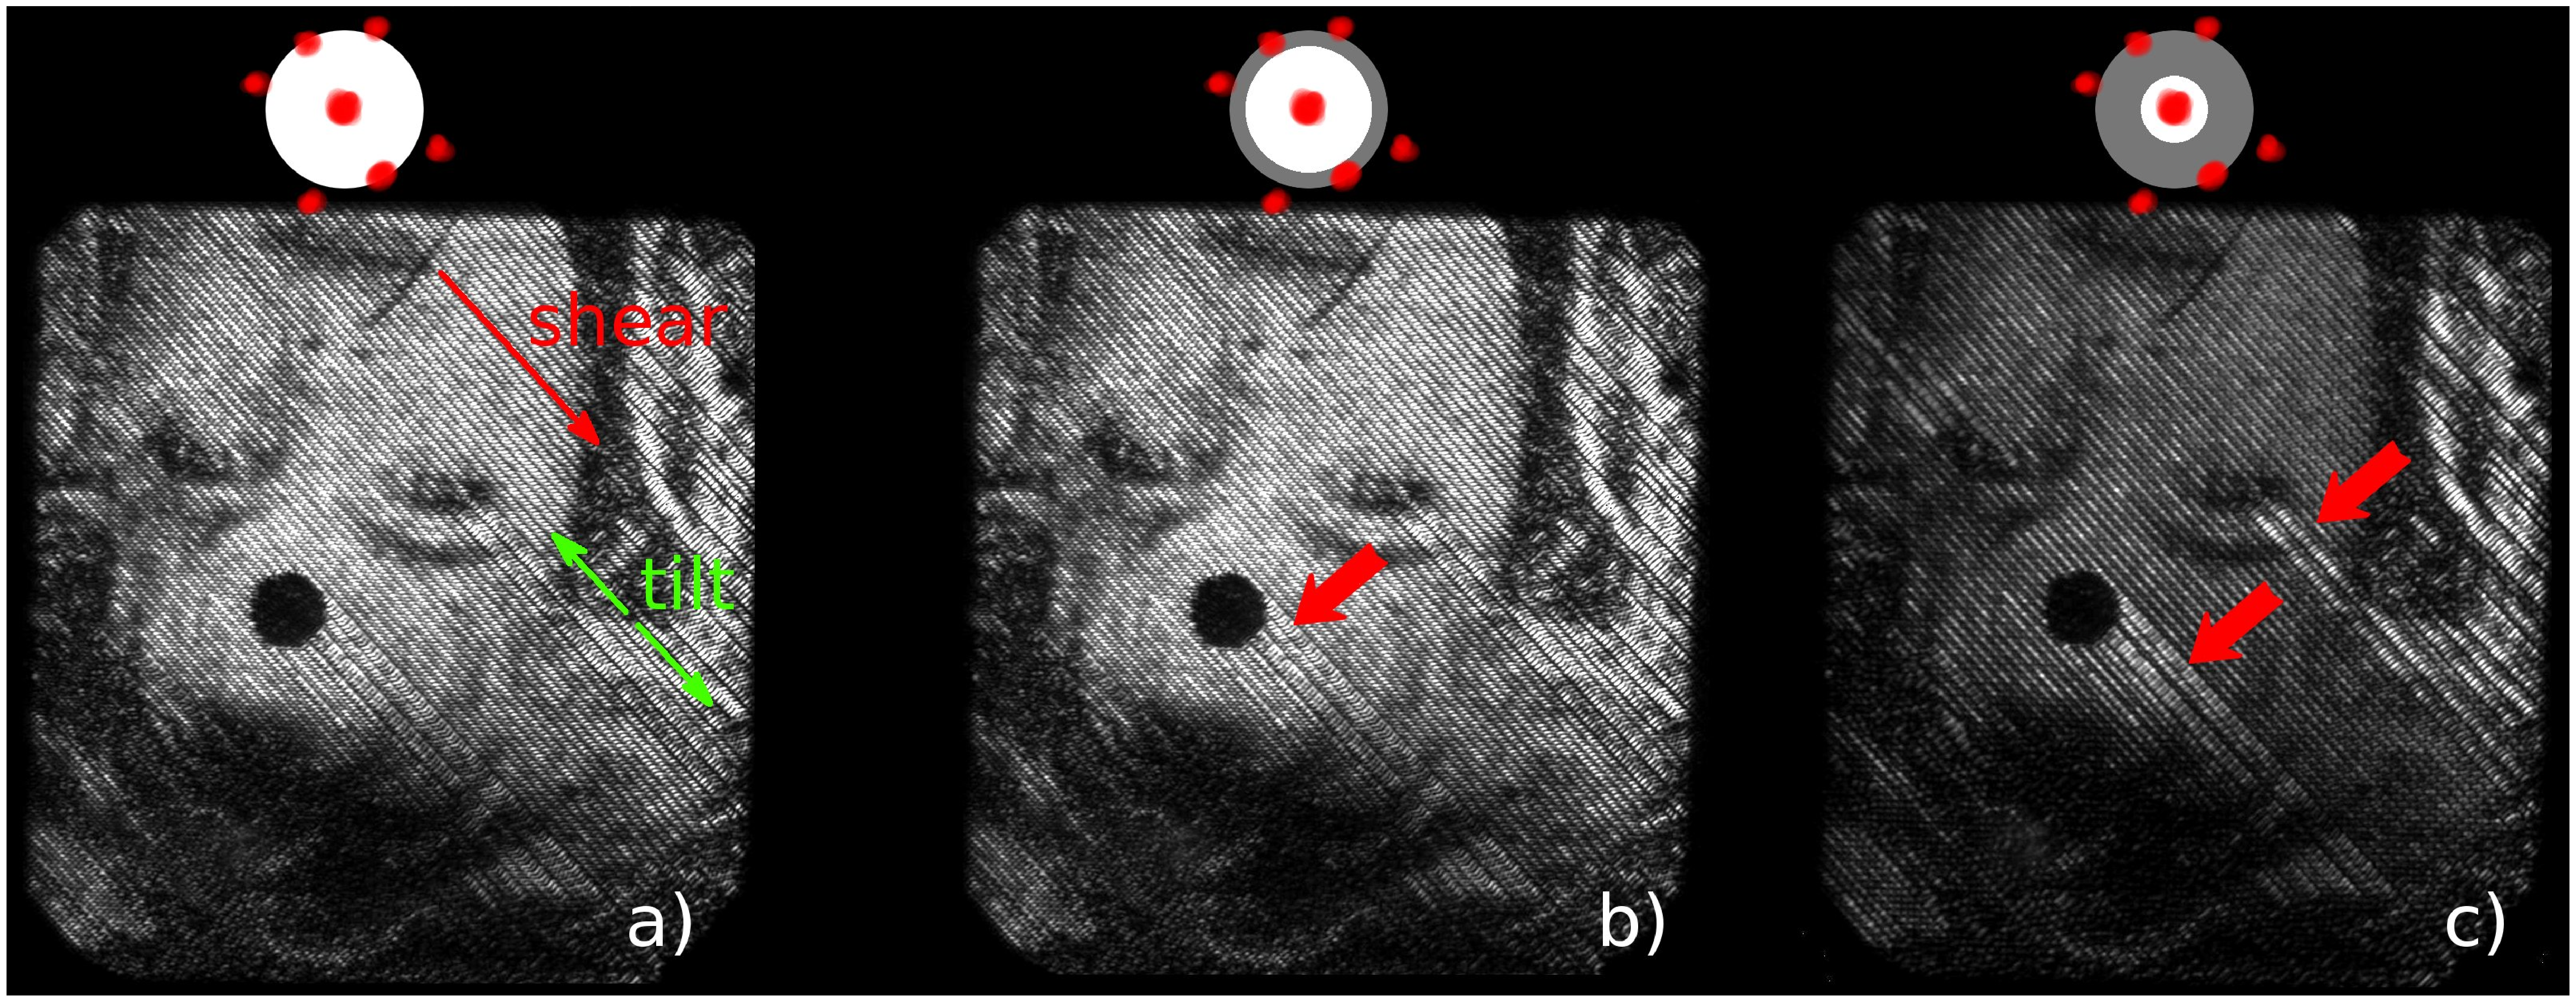
\includegraphics[width=.8\linewidth]{../app_dic/img/streaks2}
  \caption{When the $\pm1^\textrm{st}$ orders do not pass through the
    Nomarski prism, unwanted artefacts arise.  These images were
    obtained with one Nomarski prism (for $63\times/1.4$ micro
    objective) a \unit[200]{mm} objective lens and a \unit[500]{mm}
    tube lens.}
  \label{fig:erikas}
\end{figure}
\begin{figure}[!hbtp]
   \centering
   
\includegraphics[width=7cm]{../app_dic/img/1219/auswert/erika-streak-overview}
   \caption{Pattern that is displayed on the MMA for the images in
     \figref{fig:erika-detail}~c) and \figref{fig:erikas}. The shear
     direction is from top left to bottom right.}
   \label{fig:erika-streak-overview}
 \end{figure}
\section{Discussion}
We showed that a differential interference approach can be used to
convert the micro mirror array into an intensity spatial light
modulator. It is necessary that the $\pm1^\textrm{st}$ diffraction
orders contribute to the interference image. The best results were
obtained by two Nomarski prisms (each \unit[0.078]{mrad} split angle
and \unit[10]{mm} clear aperture) in series and an objective lens with
\unit[100]{mm} focal length. In this configuration the
$\pm1^\textrm{st}$ diffraction orders are $\unit[\pm2.9]{mm}$
off-axis. This leaves ca.\ $\unit[2.1]{mm}$ for illumination angles
and therefore not much more than the angular acceptence of a Fourier
filtering based approach, which could accommodate a radius of
$\unit[1.4]{mm}$.

The differential interference approach is a promising candidate to
convert piston mirror devices into intensity modulators.
